\appendix
\onecolumn

\section{Related works}
\label{sec:related works}

\textbf{Explanations for DNNs.}
Many methods have been proposed to explain DNNs, such as visualizing the features learned by the DNN~\cite{simonyan2013deep,zeiler2014visualizing,yosinski2015understanding,dosovitskiy2016inverting}, and estimating the pixel-wise attribution/saliency of input samples~\cite{Adamczewski2010bayesian,ribeiro2016should,lundberg2017unified,fong2017interpretable,zhou2014object,zhou2016learning,selvaraju2017grad}.
\cite{chen2018L2X} and \cite{yoon2019invase} estimated the smallest subset of variables to mimic DNN’s output.
Some studies extracted logical rules as explanations~\cite{ignatiev2019abduction,ignatiev2019relating,pmlr-v139-marques-silva21a,barbiero2022entropy,wang2021scalable}.
Meanwhile, another direction is to distill a DNN into another interpretable symbolic model, for example, an additive model~\cite{vaughan2018explainable,tan2018learning}, decision tree~\cite{frosst2017distilling,che2016interpretable,wu2018beyond,abroshan2023symbolic}, or graphical model~\cite{zhang2018interpreting,shih2019compiling}.
\textit{However, most of these explainer models usually only consider the model's fitness to the network output, but whether their explanation can always faithfully reflect the logic in the DNN under various data transformations is still an open problem.}
In this study, we find that the network outputs on an exponential number of randomly masked samples can always be explained by a causal graph, of which the faithfulness is theoretically proven.

\textbf{Using causality to explain DNNs.}
The causality framework was originally proposed to study the causal structure of a set of observed variables~\cite{pearl2009causality,hoyer2008nonlinear}.
For example, \cite{xia2021causal} proposed a neural-causal model to identify and estimate causal relationships in data.
Recently, several studies have explained DNNs based on causality.
For example, some studies~\cite{frye2020asymmetric,heskes2020causal,wang2021shapley} proposed attribution methods based on manually defined causal relationships between input variables.
Similarly, \cite{alvarez2017causal,harradon2018causal,chattopadhyay2019neural} explained the association between inputs and intermediate features/outputs using causal models.
Instead of manually setting or assuming causal relationships, we quantify the exact interactive concepts encoded by the DNN as causal patterns for inference, whose faithfulness is both theoretically guaranteed and experimentally verified.
Note that the SCM in Eq. (2) of the main paper does not explain the DNN as a linear model, such as a bag-of-words model~\cite{sivic2003video,csurka2004visual}.
This is because given different samples, the DNN may activate different sets of causal patterns.



\textbf{Interactions.}
Causal patterns in the proposed causal graph can actually be considered as a specific type of interaction in game theory.
Similar to causal effects, interactions in game theory are widely used to quantify the numerical effects of interactive concepts between input variables on the DNN output~\cite{sorokina2008detecting,murdoch2018beyond,singh2018hierarchical,jin2019towards,janizek2020explaining}.
In game theory, the Shapley interaction index~\cite{grabisch1999axiomatic} was used by \cite{lundberg2018consistent} to analyze tree ensembles.
\cite{sundararajan2020shapley,tsai2022faith} proposed interaction metrics from different perspectives. 
\cite{deng2022discovering} proved that DNNs were less likely to encode interactive concepts of intermediate complexity.
Unlike previous studies, we find that we can use a few causal patterns (interactive concepts) to faithfully represent the inference logic of a DNN, which is experimentally verified.



\section{Harsanyi dividend}
\label{sec:app-harsanyi-intro}


This section revisits the definition of Harsanyi dividend~\cite{harsanyi1963simplified}, a typical metric in game theory.
In this study, the causal effect {\small$w_{\mathcal{S}}$} of each pattern {\small$\mathcal{S}$} is quantified based on Harsanyi dividends.
In game theory, a complex system (\emph{e.g.,} a deep model) is usually considered a game.
Each input variable represents a player in the game, and the output of this system is the reward obtained by a subset of players.
Specifically, let us consider a deep model and an input sample {\small$\boldsymbol{x}$} with {\small$n$} variables (\emph{e.g.} a sentence with {\small$n$} words) {\small$\mathcal{N}=\{1,2,...,n\}$}.
A deep model can be understood as a game {\small$v(\cdot)$}.
In this game, the input variables in {\small$\mathcal{N}$} do not individually contribute to the model output.
Instead, they interact with each other to form concepts (causal patterns) for inference.
Each concept {\small$\mathcal{S}\subseteq\mathcal{N}$} has a certain causal effect on the model output.
In this study, we prove in Theorem \ref{th:app-harsanyi-faithful} that the Harsanyi dividend {\small$w_{\mathcal{S}}$} is a unique faithful metric for quantifying such causal effects.

\begin{small}
\begin{equation}
    w_{\mathcal{S}} = \sum_{\mathcal{S}'\subseteq\mathcal{S}} (-1)^{|\mathcal{S}'|-|\mathcal{S}|}\cdot v(\boldsymbol{x}_{\mathcal{S}'}),
\end{equation}
\end{small}

where {\small$v(\boldsymbol{x}_{\mathcal{S}})$} denotes the model output when only variables in the subset {\small$\mathcal{S}\subseteq\mathcal{N}$} are given, and all other variables are masked using their baseline values.


We also prove that the Harsanyi dividend {\small$w_{\mathcal{S}}$} satisfies seven desirable axioms, including the \textit{efficiency, linearity, dummy, symmetry, anonymity, recursive} and \textit{interaction distribution} axioms, which demonstrates its trustworthiness.

(1) \textit{Efficiency axiom}. The output score of a model can be decomposed into effects of different causal patterns, \emph{i.e.} {\small $v(\boldsymbol{x})=\sum_{\mathcal{S}\subseteq\mathcal{N}}w_{\mathcal{S}}$}.

(2) \textit{Linearity axiom}. If we merge the output scores of the two models $t(\cdot)$ and $u(\cdot)$ into the output of model $v(\cdot)$, \emph{i.e.} {\small $\forall \mathcal{S}\subseteq\mathcal{N},~ v(\boldsymbol{x}_{\mathcal{S}})=t(\boldsymbol{x}_{\mathcal{S}})+u(\boldsymbol{x}_{\mathcal{S}})$}, the corresponding causal effects {\small $w^t_{\mathcal{S}}$} and {\small $w^u_{\mathcal{S}}$} can also be merged as {\small$\forall \mathcal{S}\subseteq \mathcal{N}, w^v_{\mathcal{S}}=w^t_{\mathcal{S}}+w^u_{\mathcal{S}}$}.

(3) \textit{Dummy axiom}. If a variable {\small $i\in\mathcal{N}$} is a dummy variable, \emph{i.e.} 
{\small $\forall \mathcal{S}\subseteq \mathcal{N}\backslash\{i\}, v(\boldsymbol{x}_{\mathcal{S}\cup\{i\}})=v(\boldsymbol{x}_{\mathcal{S}})+v(\boldsymbol{x}_{\{i\}})$}, it has no causal effect with other variables, {\small $\forall \mathcal{S}\subseteq \mathcal{N}\backslash\{i\}, w_{\mathcal{S}\cup\{i\}}=0$}.

(4) \textit{Symmetry axiom}. If the input variables {\small $i,j\in \mathcal{N}$} cooperate with other variables in the same manner, {\small $\forall \mathcal{S}\subseteq \mathcal{N}\backslash\{i,j\}, v(\boldsymbol{x}_{\mathcal{S}\cup\{i\}})=v(\boldsymbol{x}_{\mathcal{S}\cup\{j\}})$}, then they have the same causal effects with other variables, {\small $\forall S\subseteq \mathcal{N}\backslash\{i,j\}, w_{\mathcal{S}\cup\{i\}}=w_{\mathcal{S}\cup\{j\}}$}.

(5) \textit{Anonymity axiom}. For any permutations $\pi$ on {\small $\mathcal{N}$}, we have {\small $\forall \mathcal{S}
\!\subseteq\! \mathcal{N}, w^v_{\mathcal{S}}\!=\!w^{\pi v}_{\pi \mathcal{S}}$}, where {\small $\pi \mathcal{S} \!\triangleq\!\{\pi(i)|i\!\in\!\! \mathcal{S}\}$}, and the new model {\small $\pi v$} is defined by {\small $(\pi v)(\boldsymbol{x}_{\pi\mathcal{S}})\!=\!v(\boldsymbol{x}_{\mathcal{S}})$}.
This indicates that causal effects are not changed by the permutation.

(6) \textit{Recursive axiom}. The causal effects can be computed recursively.
For {\small $i\in \mathcal{N}$} and {\small $\mathcal{S}\subseteq \mathcal{N}\backslash\{i\}$}, the causal effect of the pattern {\small $\mathcal{S}\cup\{i\}$} is equal to the causal effect of {\small $\mathcal{S}$} in the presence of $i$ minus the causal effect of $\mathcal{S}$ in the absence of $i$, \emph{i.e.} {\small $\forall \mathcal{S}\!\subseteq\! \mathcal{N}\!\setminus\!\{i\}, w_{\mathcal{S}\cup\{i\}} = w_{\mathcal{S}|i~\text{present}} - w_{\mathcal{S}}$}. {\small $w_{\mathcal{S}|i~\text{present}}$} denotes the causal effect when the variable $i$ is always present as a constant context, \emph{i.e.} {\small $
w_{\mathcal{S}|i~\text{present}}=\sum_{\mathcal{S}'\subseteq \mathcal{S}} (-1)^{|\mathcal{S}|-|\mathcal{S}'|}\cdot v(\boldsymbol{x}_{\mathcal{S}'\cup\{i\}})$}.

(7) \textit{Interaction distribution axiom}. This axiom characterizes how causal effects are distributed for a class of ``interaction functions''~\cite{sundararajan2020shapley}.
The interaction function {\small $v_{\mathcal{T}}$} parameterized by a subset of variables {\small $\mathcal{T}$} is defined as follows.
{\small $\forall \mathcal{S}\subseteq \mathcal{N}$}, if {\small $\mathcal{T}\subseteq \mathcal{S}$}, {\small$v_{\mathcal{T}}(\boldsymbol{x}_{\mathcal{S}})=c$}; otherwise, {\small $v_{\mathcal{T}}(\boldsymbol{x}_{\mathcal{S}})=0$}.
The function {\small$v_{\mathcal{T}}$} models the causal effect of the pattern {\small$\mathcal{T}$}, because only if all variables in {\small$\mathcal{T}$} are present, will the output value be increased by {\small$c$}.
The causal effects encoded in the function {\small$v_{\mathcal{T}}$} satisfy {\small $w_{\mathcal{T}}=c$}, and {\small $\forall \mathcal{S}\neq \mathcal{T}$}, {\small $w_{\mathcal{S}}=0$}.

More crucially, we  also prove that causal effects {\small$w_{\mathcal{S}}$} based on the Harsanyi dividend can explain the elementary mechanism of existing game-theoretic attributions/interactions, as follows.


\begin{manualtheorem}{5}[Theorem 5 {\normalfont (Connection to the marginal benefit~\cite{grabisch1999axiomatic})}]\label{th:harsanyi-marginal-benefit}
Let {\small $\Delta v_{\mathcal{T}}(\boldsymbol{x}_{\mathcal{S}})=\sum_{\mathcal{T}'\subseteq \mathcal{T}}(-1)^{|\mathcal{T}|-|\mathcal{T}'|}v(\boldsymbol{x}_{\mathcal{T}'\cup \mathcal{S}})$} denote the marginal benefit of variables in {\small $\mathcal{T}\subseteq \mathcal{N}\setminus \mathcal{S}$} given the environment {\small $\mathcal{S}$}. We have proven that {\small $\Delta v_{\mathcal{T}}(\boldsymbol{x}_{\mathcal{S}})$} can be decomposed into the sum of the causal effects inside {\small $\mathcal{T}$} and the sub-environments of {\small $\mathcal{S}$}, \emph{i.e.} {\small $\Delta v_{\mathcal{T}}(\boldsymbol{x}_{\mathcal{S}})=\sum_{\mathcal{S}'\subseteq \mathcal{S}}w_{\mathcal{T}\cup \mathcal{S}'}$}.
\end{manualtheorem}


\begin{manualtheorem}{2}[Theorem 2 {\normalfont (Connection to the Shapley value~\cite{shapley1953value})}]\label{th:app-harsanyi-shapley-value}
Let {\small $\phi(i)$} denote the Shapley value of input variable $i$.
Then, the Shapley value {\small$\phi(i)$} can be explained as the result of uniformly assigning causal effects to each involved variable {\small$i$}, \emph{i.e.}, {\small $\phi(i)=\sum_{\mathcal{S}\subseteq \mathcal{N}\backslash\{i\}}\frac{1}{|\mathcal{S}|+1} w_{\mathcal{S}\cup\{i\}}$}.
\emph{This theorem also proves that the Shapley value is a fair assignment of attributions from the perspective of causal effects.
}
\end{manualtheorem}

\begin{manualtheorem}{3}[Theorem 3 {\normalfont (Connection to the Shapley interaction index~\cite{grabisch1999axiomatic})}]\label{th:harsanyi-shapley-interaction}
Given a subset of input variables {\small $\mathcal{T} \subseteq \mathcal{N}$}, the Shapley interaction index {\small$I^{\textrm{Shapley}}(\mathcal{T})$} can be represented as {\small $I^{\textrm{Shapley}}(\mathcal{T})=\sum_{\mathcal{S}\subseteq \mathcal{N} \backslash\mathcal{T}}\frac{1}{|\mathcal{S}|+1}w_{\mathcal{S}\cup \mathcal{T}}$}.
In other words, the index {\small$I^{\textrm{Shapley}}(\mathcal{T})$} can be explained as uniformly allocating causal effects {\small$w_{\mathcal{S}'}$} s.t. {\small$\mathcal{S}'=\mathcal{S}\cup \mathcal{T}$} to the compositional variables of {\small$\mathcal{S}'$}, if we treat the coalition of variables in {\small $\mathcal{T}$} as a single variable.
\end{manualtheorem}

\begin{manualtheorem}{4}[Theorem 4 {\normalfont (Connection to the Shapley Taylor interaction index~\cite{sundararajan2020shapley})}]\label{th:harsanyi-shapley-taylor}
Given a subset of input variables {\small $\mathcal{T}\subseteq \mathcal{N}$}, the {\small$k$}-th order Shapley Taylor interaction index {\small $I^{\textrm{Shapley-Taylor}}(\mathcal{T})$} can be represented as weighted sum of causal effects, \emph{i.e.}, {\small $I^{\textrm{Shapley-Taylor}}(\mathcal{T})=w_{\mathcal{T}}$} if {\small $|\mathcal{T}|<k$}; {\small $I^{\textrm{Shapley-Taylor}}(\mathcal{T})=\sum_{\mathcal{S}\subseteq \mathcal{N}\backslash \mathcal{T}}\binom{|\mathcal{S}|+k}{k}^{-1}w_{\mathcal{S}\cup \mathcal{T}}$} if {\small $|\mathcal{T}|=k$}; and {\small $I^{\textrm{Shapley-Taylor}}(\mathcal{T})=0$ if $|\mathcal{T}|>k$}.
\end{manualtheorem}




\section{The proof of Theorem \ref{th:app-harsanyi-faithful} in the main paper}
\label{sec:app-proof-harsanyi-faithful}

\begin{manualtheorem}{1}[Theorem 1]\label{th:app-harsanyi-faithful}
Given a certain input {\small$\boldsymbol{x}$}, let the causal graph in Fig. 1 (in the main paper) encode {\small$2^n$} causal patterns, \emph{i.e.}, {\small$\Omega=2^{\mathcal{N}}=\{\mathcal{S}: \mathcal{S}\subseteq\mathcal{N}\}$}.
If the causal effect {\small$w_{\mathcal{S}}$} of each causal pattern {\small$\mathcal{S}\in\Omega$} is measured by the Harsanyi dividend~\cite{harsanyi1963simplified}, \emph{i.e.} {\small$w_{\mathcal{S}} \triangleq {\sum}_{\mathcal{S}'\subseteq \mathcal{S}}(-1)^{|\mathcal{S}|-|\mathcal{S}'|}\cdot v(\boldsymbol{x}_{\mathcal{S}'})$}, then the causal graph faithfully encodes the inference logic of the DNN, as follows.


\vspace{-5pt}
\begin{small}
\begin{equation}
    \forall \mathcal{S}\subseteq \mathcal{N},\ \ 
    Y(\boldsymbol{x}_{\mathcal{S}}) = v(\boldsymbol{x}_{\mathcal{S}})
\end{equation}
\end{small}
More crucially, the Harsanyi dividend is the unique metric that satisfies the faithfulness requirement.
\end{manualtheorem}

$\bullet$~\textit{Proof:} We only need to prove the following two statements. (1) Necessity: the causal graph based on Harsanyi dividends {\small$w_{\mathcal{S}}$} satisfies the faithfulness requirement {\small$\forall \mathcal{S}\subseteq \mathcal{N}, Y(\boldsymbol{x}_{\mathcal{S}})\!=\! v(\boldsymbol{x}_{\mathcal{S}})$}.
(2) Sufficiency: if there exists another metric {\small$\tilde{w}_{\mathcal{S}}$} that also satisfies the faithfulness requirement, then, it is equivalent to the Harsanyi dividend, \emph{i.e.} {\small$\forall \mathcal{S}\subseteq \mathcal{N}, \tilde{w}_{\mathcal{S}}=w_{\mathcal{S}}$}.

According to the SCM in Eq. (2) of the main paper, we have {\small$Y(\boldsymbol{x}_{\mathcal{S}})=\sum_{\mathcal{S}'\in\Omega}w_{\mathcal{S}'}\cdot C_{\mathcal{S}'}(\boldsymbol{x}_{\mathcal{S}})=\sum_{\mathcal{S}'\subseteq\mathcal{S}}w_{\mathcal{S}'}$}.
Therefore, the faithfulness requirement can be equivalently re-written as {\small$\forall \mathcal{S}\subseteq \mathcal{N}, v(\boldsymbol{x}_{\mathcal{S}})=\sum_{\mathcal{S}'\subseteq\mathcal{S}}w_{\mathcal{S}'}$}.

\textit{Proof for necessity.}
According to the definition of the Harsanyi dividend, we have {\small$\forall \mathcal{S}\subseteq \mathcal{N}$}, 

\begin{small}
\begin{align*}
\sum_{\mathcal{S}'\subseteq \mathcal{S}}  w_{\mathcal{S}'}  =& \sum_{\mathcal{S}'\subseteq \mathcal{S}} \sum_{\mathcal{L}\subseteq \mathcal{S}'} (-1)^{|\mathcal{S}'|-|\mathcal{L}|}  v(\boldsymbol{x}_{\mathcal{L}}) \\
=& \sum_{\mathcal{L}\subseteq \mathcal{S}} \sum_{\mathcal{S}'\subseteq \mathcal{S}: \mathcal{S}'\supseteq \mathcal{L}} (-1)^{|\mathcal{S}'|-|\mathcal{L}|} v(\boldsymbol{x}_{\mathcal{L}}) \\
=& \sum_{\mathcal{L}\subseteq \mathcal{S}} \sum_{s'=|\mathcal{L}|}^{|\mathcal{S}|} \sum_{\scriptsize\substack{\mathcal{S}'\subseteq \mathcal{S}: \mathcal{S}'\supseteq \mathcal{L}\\
|\mathcal{S}'|=s'}} (-1)^{s'-|\mathcal{L}|} v(\boldsymbol{x}_{\mathcal{L}}) \\
=& \sum_{\mathcal{L}\subseteq \mathcal{S}} v(\boldsymbol{x}_{\mathcal{L}})  \sum_{m=0}^{|\mathcal{S}|-|\mathcal{L}|} \binom{|\mathcal{S}|-|\mathcal{L}|}{m} (-1)^{m}= v(\boldsymbol{x}_{\mathcal{S}}) 
\end{align*}
\end{small}



\textit{Proof for sufficiency.}
Suppose there exists another metric {\small$\tilde{w}_{\mathcal{S}}$} that satisfies {\small$\forall \mathcal{S}\subseteq \mathcal{N}, v(\boldsymbol{x}_{\mathcal{S}})  = {\sum}_{\mathcal{S}'\subseteq \mathcal{S}} \tilde{w}_{\mathcal{S}'} $}.
Then, we prove {\small$\tilde{w}_{\mathcal{S}} = w_{\mathcal{S}} $} by induction on the number of variables {\small$|\mathcal{S}|$} in the causal pattern.



\textit{(Basis step)}
When {\small$|\mathcal{S}|=0$}, \emph{i.e.} {\small$\mathcal{S}=\emptyset$}, we have {\small$\tilde{w}_{\emptyset} = v(\boldsymbol{x}_{\emptyset}) = w_{\emptyset}$}.
Similarly, it can be directly derived that when {\small$|\mathcal{S}|=1$}, \emph{i.e.} {\small$\mathcal{S}=\{i\}$}, {\small$\tilde{w}_{\{i\}} = v(\boldsymbol{x}_{\{i\}}) - v(\boldsymbol{x}_{\emptyset}) = w_{\{i\}}$}; 
when {\small$|\mathcal{S}|=2$}, \emph{i.e.} {\small$\mathcal{S}=\{i,j\}$}, {\small$\tilde{w}_{\{i,j\}} = v(\boldsymbol{x}_{\{i,j\}}) - v(\boldsymbol{x}_{\{i\}}) - v(\boldsymbol{x}_{\{j\}}) + v(\boldsymbol{x}_{\emptyset}) = w_{\{i, j\}}$}.


\textit{(Induction step)} Suppose {\small$\tilde{w}_{\mathcal{S}} = w_{\mathcal{S}} $} holds for any {\small$\mathcal{S}$} with {\small$|\mathcal{S}|=s\geq 2$}. 
Then, for {\small$|\mathcal{S}|=s+1$}, we have

\begin{small}
\begin{align*}
 v(\boldsymbol{x}_{\mathcal{S}})  =& \sum_{\mathcal{S}'\subseteq \mathcal{S}} \tilde{w}_{\mathcal{S}'}  =  \tilde{w}_{\mathcal{S}}  + \sum_{\mathcal{S}'\subsetneq \mathcal{S}} \tilde{w}_{\mathcal{S}'} \\
=&  \tilde{w}_{\mathcal{S}}  + \sum_{\mathcal{S}'\subsetneq \mathcal{S}}\sum_{\mathcal{L}\subseteq \mathcal{S}'}(-1)^{|\mathcal{S}'|-|\mathcal{L}|} v(\boldsymbol{x}_{\mathcal{L}}) \qquad\text{// by the induction assumption}\\
=&  \tilde{w}_{\mathcal{S}}  + \sum_{\mathcal{L}\subsetneq \mathcal{S}}\sum_{\mathcal{S}'\subsetneq \mathcal{S}:\mathcal{L}\subseteq \mathcal{S}'} (-1)^{|\mathcal{S}'|-|\mathcal{L}|}\cdot  v(\boldsymbol{x}_{\mathcal{L}}) \\
=&  \tilde{w}_{\mathcal{S}}  + \sum_{\mathcal{L}\subsetneq \mathcal{S}}\sum_{s'=|\mathcal{L}|}^{|\mathcal{S}|-1}\sum_{\scriptsize\substack{\mathcal{S}'\subsetneq \mathcal{S}: \mathcal{L}\subseteq \mathcal{S}'\\|\mathcal{S}'|=s'}} (-1)^{s'-|\mathcal{L}|}\cdot  v(\boldsymbol{x}_{\mathcal{L}}) \\
=&  \tilde{w}_{\mathcal{S}}  + \sum_{\mathcal{L}\subsetneq \mathcal{S}}  v(\boldsymbol{x}_{\mathcal{L}})  \sum_{s'=|\mathcal{L}|}^{|\mathcal{S}|-1} \binom{|\mathcal{S}|-|\mathcal{L}|}{s'-|\mathcal{L}|} (-1)^{s'-|\mathcal{L}|}\\
=&  \tilde{w}_{\mathcal{S}}  + \sum_{\mathcal{L}\subsetneq \mathcal{S}}  v(\boldsymbol{x}_{\mathcal{L}})  \underbrace{\sum_{m=0}^{|\mathcal{S}|-|\mathcal{L}|-1} \binom{|\mathcal{S}|-|\mathcal{L}|}{m} (-1)^{m}}_{0-(-1)^{|\mathcal{S}|-|\mathcal{L}|}}\\
=&  \tilde{w}_{\mathcal{S}}  - \sum_{\mathcal{L}\subsetneq \mathcal{S}}(-1)^{|\mathcal{S}|-|\mathcal{L}|}  v(\boldsymbol{x}_{\mathcal{L}}) .
\end{align*}
\end{small}

In this way, we have 
\begin{small}
\begin{equation*}
     \tilde{w}_{\mathcal{S}}  =  v(\boldsymbol{x}_{\mathcal{S}})  + \sum_{\mathcal{L}\subsetneq \mathcal{S}}(-1)^{|\mathcal{S}|-|\mathcal{L}|}  v(\boldsymbol{x}_{\mathcal{L}})  = \sum_{\mathcal{L}\subseteq \mathcal{S}}(-1)^{|\mathcal{S}|-|\mathcal{L}|} v(\boldsymbol{x}_{\mathcal{L}})  =  w_{\mathcal{S}} .
\end{equation*}
\end{small}

Therefore, the Harsanyi dividend is \textbf{the unique metric} that satisfies the faithfulness requirement.

\section{Proofs of axioms and theorems for the Harsanyi dividend}
\label{sec:app-proof-harsanyi-property}

\subsection{Proofs of axioms}
\label{sec:app-interaction-axioms}

In this section, we prove that the Harsanyi dividend {\small$w_{\mathcal{S}}$} satisfies the \emph{efficiency, linearity, dummy, symmetry, anonymity, recursive,} and \emph{interaction distribution} axioms.

\textbf{(1) Efficiency axiom.} The output score of a model can be decomposed into effects of different causal patterns, \emph{i.e.} {\small $v(\boldsymbol{x})=\sum_{\mathcal{S}\subseteq\mathcal{N}}w_{\mathcal{S}}$}.

$\bullet$~\textit{Proof:} According to the definition of the Harsanyi dividend, we have

\begin{small}
\begin{align*}
\sum_{\mathcal{S}\subseteq \mathcal{N}} w_{\mathcal{S}} 
=& \sum_{\mathcal{S}\subseteq \mathcal{N}} \sum_{\mathcal{S}'\subseteq \mathcal{S}} (-1)^{|\mathcal{S}|-|\mathcal{S}'|}\cdot v(\boldsymbol{x}_{\mathcal{S}'})\\
=& \sum_{\mathcal{S}'\subseteq \mathcal{N}} \sum_{\scriptsize\mathcal{S}:\mathcal{S}'\subseteq\mathcal{S}\subseteq\mathcal{N}} (-1)^{|\mathcal{S}|-|\mathcal{S}'|}\cdot v(\boldsymbol{x}_{\mathcal{S}'})\\
=& \sum_{\mathcal{S}'\subseteq \mathcal{N}} \sum_{s=|\mathcal{S}'|}^{n} \sum_{\scriptsize\substack{\mathcal{S}:\mathcal{S}'\subseteq\mathcal{S}\subseteq\mathcal{N}\\
|\mathcal{S}|=s}} (-1)^{s-|\mathcal{S}'|}v(\boldsymbol{x}_{\mathcal{S}'})\\
=& \sum_{\mathcal{S}'\subseteq \mathcal{N}}v(\boldsymbol{x}_{\mathcal{S}'}) \sum_{m=0}^{n-|\mathcal{S}'|} \binom{n-|\mathcal{S}'|}{m} (-1)^{m}\\
=& v(\boldsymbol{x}) \quad\text{// the only case that cannot be cancelled out is {\small$\mathcal{S}'=\mathcal{N}$}}
\end{align*}
\end{small}



\textbf{(2) Linearity axiom.} If we merge output scores of two models $t(\cdot)$ and $u(\cdot)$ as the output of model $v(\cdot)$, \emph{i.e.} {\small $\forall \mathcal{S}\subseteq\mathcal{N},~ v(\boldsymbol{x}_{\mathcal{S}})=t(\boldsymbol{x}_{\mathcal{S}})+u(\boldsymbol{x}_{\mathcal{S}})$}, then the corresponding causal effects {\small $w^t_{\mathcal{S}}$} and {\small $w^u_{\mathcal{S}}$} can also be merged as {\small$\forall \mathcal{S}\subseteq \mathcal{N}, w^v_{\mathcal{S}}=w^t_{\mathcal{S}}+w^u_{\mathcal{S}}$}.

$\bullet$~\textit{Proof:} According to the definition of the Harsanyi dividend, we have

\begin{small}
\begin{align*}
w^v_{\mathcal{S}} =& \sum_{\mathcal{S}'\subseteq \mathcal{S}}(-1)^{|\mathcal{S}|-|\mathcal{S}'|}v(\boldsymbol{x}_{\mathcal{S}})\\
=& \sum_{\mathcal{S}'\subseteq \mathcal{S}}(-1)^{|\mathcal{S}|-|\mathcal{S}'|}[t(\boldsymbol{x}_{\mathcal{S}})+u(\boldsymbol{x}_{\mathcal{S}})]\\
=&\sum_{\mathcal{S}'\subseteq \mathcal{S}}(-1)^{|\mathcal{S}|-|\mathcal{S}'|}t(\boldsymbol{x}_{\mathcal{S}})+\sum_{\mathcal{S}'\subseteq \mathcal{S}}(-1)^{|\mathcal{S}|-|\mathcal{S}'|}u(\boldsymbol{x}_{\mathcal{S}})\\
=& w^t_{\mathcal{S}}+w^u_{\mathcal{S}}.
\end{align*}
\end{small}

\textbf{(3) Dummy axiom.} If a variable {\small $i\in\mathcal{N}$} is a dummy variable, \emph{i.e.} 
{\small $\forall \mathcal{S}\subseteq \mathcal{N}\backslash\{i\}, v(\boldsymbol{x}_{\mathcal{S}\cup\{i\}})=v(\boldsymbol{x}_{\mathcal{S}})+v(\boldsymbol{x}_{\{i\}})$}, then it has no causal effect with other variables, {\small $\forall \mathcal{S}\subseteq \mathcal{N}\backslash\{i\}, w_{\mathcal{S}\cup\{i\}}=0$}.

$\bullet$~\textit{Proof:} According to the definition of the Harsanyi dividend, we have

\begin{small}
\begin{align*}
w_{\mathcal{S}\cup\{i\}} =& \sum_{\mathcal{S}'\subseteq \mathcal{S}\cup\{i\}} (-1)^{|\mathcal{S}|+1-|\mathcal{S}'|}v(\boldsymbol{x}_{\mathcal{S}'})\\
=& \sum_{\mathcal{S}'\subseteq \mathcal{S}} (-1)^{|\mathcal{S}|+1-|\mathcal{S}'|}v(\boldsymbol{x}_{\mathcal{S}'}) + \sum_{\mathcal{S}'\subseteq \mathcal{S}} (-1)^{|\mathcal{S}|-|\mathcal{S}'|}v(\boldsymbol{x}_{\mathcal{S}'\cup\{i\}})\\
=& \sum_{\mathcal{S}'\subseteq \mathcal{S}} (-1)^{|\mathcal{S}|+1-|\mathcal{S}'|}v(\boldsymbol{x}_{\mathcal{S}'}) + \sum_{\mathcal{S}'\subseteq \mathcal{S}} (-1)^{|\mathcal{S}|-|\mathcal{S}'|}[v(\boldsymbol{x}_{\mathcal{S}})+v(\boldsymbol{x}_{\{i\}})]\\
=& \Big[\sum_{\mathcal{S}'\subseteq \mathcal{S}}(-1)^{|\mathcal{S}|-|\mathcal{S}'|}\Big]\cdot v(\boldsymbol{x}_{\{i\}})\\
=& 0.
\end{align*}
\end{small}

\textbf{(4) Symmetry axiom.} If input variables {\small $i,j\in \mathcal{N}$} cooperate with other variables in the same way, {\small $\forall \mathcal{S}\subseteq \mathcal{N}\backslash\{i,j\}, v(\boldsymbol{x}_{\mathcal{S}\cup\{i\}})=v(\boldsymbol{x}_{\mathcal{S}\cup\{j\}})$}, then they have same causal effects with other variables, {\small $\forall S\subseteq \mathcal{N}\backslash\{i,j\}, w_{\mathcal{S}\cup\{i\}}=w_{\mathcal{S}\cup\{j\}}$}.

$\bullet$~\textit{Proof:} According to the definition of the Harsanyi dividend, we have

\begin{small}
\begin{align*}
w_{\mathcal{S}\cup\{i\}} =& \sum_{\mathcal{S}'\subseteq \mathcal{S}\cup\{i\}} (-1)^{|\mathcal{S}|+1-|\mathcal{S}'|}v(\boldsymbol{x}_{\mathcal{S}'})\\
=& \sum_{\mathcal{S}'\subseteq \mathcal{S}} (-1)^{|\mathcal{S}|+1-|\mathcal{S}'|}v(\boldsymbol{x}_{\mathcal{S}'}) + \sum_{\mathcal{S}'\subseteq \mathcal{S}} (-1)^{|\mathcal{S}|-|\mathcal{S}'|}v(\boldsymbol{x}_{\mathcal{S}'\cup\{i\}})\\
=& \sum_{\mathcal{S}'\subseteq \mathcal{S}} (-1)^{|\mathcal{S}|+1-|\mathcal{S}'|}v(\boldsymbol{x}_{\mathcal{S}'}) + \sum_{\mathcal{S}'\subseteq \mathcal{S}} (-1)^{|\mathcal{S}|-|\mathcal{S}'|}v(\boldsymbol{x}_{\mathcal{S}'\cup\{j\}})\\
=& \sum_{\mathcal{S}'\subseteq \mathcal{S}\cup\{j\}} (-1)^{|\mathcal{S}|+1-|\mathcal{S}'|}v(\boldsymbol{x}_{\mathcal{S}'})\\
=& w_{\mathcal{S}\cup\{j\}}.
\end{align*}
\end{small}

\textbf{(5) Anonymity axiom.} For any permutations $\pi$ on {\small $\mathcal{N}$}, we have {\small $\forall \mathcal{S}
\!\subseteq\! \mathcal{N}, w^v_{\mathcal{S}}\!=\!w^{\pi v}_{\pi \mathcal{S}}$}, where {\small $\pi \mathcal{S} \!\triangleq\!\{\pi(i)|i\!\in\! \mathcal{S}\}$}, and the new model {\small $\pi v$} is defined by {\small $(\pi v)(\boldsymbol{x}_{\pi\mathcal{S}})\!=\!v(\boldsymbol{x}_{\mathcal{S}})$}.
This indicates that causal effects are not changed by permutation.

$\bullet$~\textit{Proof:} According to the definition of the Harsanyi dividend, we have

\begin{small}
\begin{align*}
w^{\pi v}_{\pi \mathcal{S}}=& \sum_{\mathcal{S}'\subseteq \mathcal{S}} (-1)^{|\mathcal{S}|-|\mathcal{S}'|} (\pi v)(\boldsymbol{x}_{\pi\mathcal{S}'})\\
=& \sum_{\mathcal{S}'\subseteq \mathcal{S}} (-1)^{|\mathcal{S}|-|\mathcal{S}'|} v(\boldsymbol{x}_{\mathcal{S}'})\\
=& w^v_{\mathcal{S}}.
\end{align*}
\end{small}

\textbf{(6) Recursive axiom.} The causal effects can be computed recursively.
For {\small $i\in \mathcal{N}$} and {\small $\mathcal{S}\subseteq \mathcal{N}\backslash\{i\}$}, the causal effect of the pattern {\small $\mathcal{S}\cup\{i\}$} is equal to the causal effect of {\small $\mathcal{S}$} with the presence of $i$ minus the causal effect of $\mathcal{S}$ with the absence of $i$, \emph{i.e.} {\small $\forall \mathcal{S}\!\subseteq\! \mathcal{N}\!\setminus\!\{i\}, w_{\mathcal{S}\cup\{i\}} = w_{\mathcal{S}|i~\text{present}} - w_{\mathcal{S}}$}. {\small $w_{\mathcal{S}|i~\text{present}}$} denotes the causal effect when the variable $i$ is always present as a constant context, \emph{i.e.} {\small $
w_{\mathcal{S}|i~\text{present}}=\sum_{\mathcal{S}'\subseteq \mathcal{S}} (-1)^{|\mathcal{S}|-|\mathcal{S}'|}\cdot v(\boldsymbol{x}_{\mathcal{S}'\cup\{i\}})$}.

$\bullet$~\textit{Proof:} According to the definition of the Harsanyi dividend, we have


\begin{small}
\begin{align*}
w_{\mathcal{S}\cup\{i\}} =& \sum_{\mathcal{S}'\subseteq \mathcal{S}\cup\{i\}} (-1)^{|\mathcal{S}|+1-|\mathcal{S}'|}v(\boldsymbol{x}_{\mathcal{S}'})\\
=& \sum_{\mathcal{S}'\subseteq \mathcal{S}} (-1)^{|\mathcal{S}|+1-|\mathcal{S}'|}v(\boldsymbol{x}_{\mathcal{S}'}) + \sum_{\mathcal{S}'\subseteq \mathcal{S}} (-1)^{|\mathcal{S}|-|\mathcal{S}'|}v(\boldsymbol{x}_{\mathcal{S}'\cup\{i\}})\\
=& \sum_{\mathcal{S}'\subseteq \mathcal{S}} (-1)^{|\mathcal{S}|-|\mathcal{S}'|}v(\boldsymbol{x}_{\mathcal{S}'\cup\{i\}}) - \sum_{\mathcal{S}'\subseteq \mathcal{S}} (-1)^{|\mathcal{S}|-|\mathcal{S}'|}v(\boldsymbol{x}_{\mathcal{S}'})\\
=& w_{\mathcal{S}|i~\text{present}} - w_{\mathcal{S}}.
\end{align*}
\end{small}

\textbf{(7) Interaction distribution axiom.} This axiom characterizes how causal effects are distributed for a class of ``interaction functions''~\cite{sundararajan2020shapley}.
An interaction function {\small $v_{\mathcal{T}}$} parameterized by a subset of variables {\small $\mathcal{T}$} is defined as follows.
{\small $\forall \mathcal{S}\subseteq \mathcal{N}$}, if {\small $\mathcal{T}\subseteq \mathcal{S}$}, {\small$v_{\mathcal{T}}(\boldsymbol{x}_{\mathcal{S}})=c$}; otherwise, {\small $v_{\mathcal{T}}(\boldsymbol{x}_{\mathcal{S}})=0$}.
The function {\small$v_{\mathcal{T}}$} purely models the causal effect of the pattern {\small$\mathcal{T}$}, because only if all variables in {\small$\mathcal{T}$} are present, the output value will be increased by {\small$c$}.
The causal effects encoded in the function {\small$v_{\mathcal{T}}$} satisfy {\small $w_{\mathcal{T}}=c$}, and {\small $\forall \mathcal{S}\neq \mathcal{T}$}, {\small $w_{\mathcal{S}}=0$}.

$\bullet$~\textit{Proof:} If {\small$\mathcal{S}\subsetneq \mathcal{T}$}, we have


\begin{small}
\begin{equation*}
w_{\mathcal{S}}=\sum_{\mathcal{S}'\subseteq \mathcal{S}} (-1)^{|\mathcal{S}|-|\mathcal{S}'|}\cdot \underbrace{v(\boldsymbol{x}_{\mathcal{S}'})}_{\forall \mathcal{S}'\subseteq \mathcal{S}\subsetneq \mathcal{T}, v(\boldsymbol{x}_{\mathcal{S}'})=0}=0.
\end{equation*}
\end{small}

If {\small$\mathcal{S}= \mathcal{T}$}, we have


\begin{small}
\begin{align*}
w_{\mathcal{S}}=& w_{\mathcal{T}} = \sum_{\mathcal{S}'\subseteq \mathcal{T}}(-1)^{|\mathcal{T}|-|\mathcal{S}'|}v(\boldsymbol{x}_{\mathcal{S}'})\\
=& v(\mathcal{T}) + \sum_{\mathcal{S}'\subsetneq \mathcal{T}}(-1)^{|\mathcal{T}|-|\mathcal{S}'|}\underbrace{v(\boldsymbol{x}_{\mathcal{S}'})}_{=0}
=c.
\end{align*}
\end{small}

If {\small$\mathcal{S}\supsetneq \mathcal{T}$}, we have


\begin{small}
\begin{align*}
w_{\mathcal{S}}=& \sum_{\mathcal{S}'\subseteq \mathcal{S}}(-1)^{|\mathcal{S}|-|\mathcal{S}'|}v(\boldsymbol{x}_{\mathcal{S}'})\\
=& c\cdot\sum_{\scriptsize\substack{\mathcal{S}'\subseteq \mathcal{S}\\\mathcal{S}'\supseteq \mathcal{T}}} (-1)^{|\mathcal{S}|-|\mathcal{S}'|}\\
=& c\cdot\sum_{m=0}^{|\mathcal{S}|-|\mathcal{T}|}\binom{|\mathcal{S}|-|\mathcal{T}|}{m} (-1)^m = 0.
\end{align*}
\end{small}

\subsection{Proofs of theorems}
\label{sec:app-interaction-theorems}

In this section, we prove connections between the Harsanyi dividend {\small$w_{\mathcal{S}}$} and several game-theoretic attributions/interactions.
We first prove Theorem \ref{th:harsanyi-marginal-benefit}, which can be seen as the foundation for proofs of Theorem \ref{th:app-harsanyi-shapley-value}, \ref{th:harsanyi-shapley-interaction}, and \ref{th:harsanyi-shapley-taylor}. 



\noindent\textbf{Theorem \ref{th:harsanyi-marginal-benefit} (Connection to the marginal benefit).} Let {\small $\Delta v_{\mathcal{T}}(\boldsymbol{x}_{\mathcal{S}})=\sum_{\mathcal{T}'\subseteq \mathcal{T}}(-1)^{|\mathcal{T}|-|\mathcal{T}'|}v(\boldsymbol{x}_{\mathcal{T}'\cup \mathcal{S}})$} denote the marginal benefit of variables in {\small $\mathcal{T}\subseteq \mathcal{N}\setminus \mathcal{S}$} given the environment {\small $\mathcal{S}$}. We have proven that {\small $\Delta v_{\mathcal{T}}(\boldsymbol{x}_{\mathcal{S}})$} can be decomposed into the sum of causal effects inside {\small $\mathcal{T}$} and sub-environments of {\small $\mathcal{S}$}, \emph{i.e.} {\small $\Delta v_{\mathcal{T}}(\boldsymbol{x}_{\mathcal{S}})=\sum_{\mathcal{S}'\subseteq \mathcal{S}}w_{\mathcal{T}\cup \mathcal{S}'}$}.


$\bullet$~\textit{Proof:} By the definition of the marginal benefit, we have


\begin{small}
\begin{align*}
\Delta v_{\mathcal{T}}(\boldsymbol{x}_{\mathcal{S}})
=& \sum_{\mathcal{L}\subseteq \mathcal{T}}(-1)^{|\mathcal{T}|-|\mathcal{L}|}v(\boldsymbol{x}_{\mathcal{L}\cup\mathcal{S}})\\
=& \sum_{\mathcal{L}\subseteq \mathcal{T}} (-1)^{|\mathcal{T}|-|\mathcal{L}|}\sum_{\mathcal{K}\subseteq \mathcal{L}\cup \mathcal{S}} w_{\mathcal{K}} \quad\text{// by Theorem \ref{th:app-harsanyi-faithful}}\\
=& \sum_{\mathcal{L}\subseteq \mathcal{T}} (-1)^{|\mathcal{T}|-|\mathcal{L}|}\sum_{\mathcal{L}'\subseteq \mathcal{L}}\sum_{\mathcal{S}'\subseteq \mathcal{S}} w_{\mathcal{L}'\cup \mathcal{S}'} \quad\text{// since $\mathcal{L}\cap \mathcal{S}=\emptyset$}\\
=& \sum_{\mathcal{S}'\subseteq \mathcal{S}}\left[\sum_{\mathcal{L}\subseteq \mathcal{T}} (-1)^{|\mathcal{T}|-|\mathcal{L}|} \sum_{\mathcal{L}'\subseteq \mathcal{L}} w_{\mathcal{L}'\cup \mathcal{S}'}\right]\\
=& \sum_{\mathcal{S}'\subseteq \mathcal{S}}\left[\sum_{\mathcal{L}'\subseteq \mathcal{T}}\sum_{\substack{\mathcal{L}\subseteq \mathcal{T}\\ \mathcal{L}\supseteq \mathcal{L}'}}(-1)^{|\mathcal{T}|-|\mathcal{L}|}w_{\mathcal{L}'\cup \mathcal{S}'}\right]\\
=& \sum_{\mathcal{S}'\subseteq \mathcal{S}}\left[\underbrace{w_{\mathcal{S}'\cup \mathcal{T}}}_{\mathcal{L}'=\mathcal{T}} + \underbrace{\sum_{\mathcal{L}'\subsetneq \mathcal{T}}\left(\sum_{l=|\mathcal{L}'|}^{|\mathcal{T}|}\binom{|\mathcal{T}|-|\mathcal{L}'|}{l-|\mathcal{L}'|}(-1)^{|\mathcal{T}|-|\mathcal{L}|}w_{\mathcal{L}'\cup \mathcal{S}'}\right)}_{L'\subsetneq \mathcal{T}}\right]\\
=& \sum_{\mathcal{S}'\subseteq \mathcal{S}}\left[w_{\mathcal{S}'\cup \mathcal{T}} + \sum_{\mathcal{L}'\subsetneq \mathcal{T}}\left(w_{\mathcal{L}'\cup \mathcal{S}'}\cdot\underbrace{\sum_{l=|\mathcal{L}'|}^{|\mathcal{T}|}\binom{|\mathcal{T}|-|\mathcal{L}'|}{l-|\mathcal{L}'|}(-1)^{|\mathcal{T}|-|\mathcal{L}|}}_{=0}\right)\right]\\
=& \sum_{\mathcal{S}'\subseteq \mathcal{S}} w_{\mathcal{S}'\cup \mathcal{T}}
\qed
\end{align*}
\end{small}

In particular, if {\small$\mathcal{T}$} is a singleton set, \emph{i.e.} {\small$\mathcal{T}=\{i\}$}, we can obtain a similar conclusion to \cite{ren2021learning} that {\small$\Delta v_{\{i\}}(\boldsymbol{x}_{\mathcal{S}})=\sum_{\mathcal{L}\subseteq \mathcal{S}} w_{\mathcal{L}\cup\{i\}}$}.


\vspace{5pt}
\noindent\textbf{Theorem \ref{th:app-harsanyi-shapley-value} (Connection to the Shapley value).} Let {\small $\phi(i)$} denote the Shapley value~\cite{shapley1953value} of an input variable $i$.
Then, the Shapley value {\small$\phi(i)$} can be represented as a weighted sum of causal effects involving the variable {\small$i$}, \emph{i.e.}, {\small $\phi(i)=\sum_{\mathcal{S}\subseteq \mathcal{N}\backslash\{i\}}\frac{1}{|\mathcal{S}|+1} w_{\mathcal{S}\cup\{i\}}$}.
\textit{In other words, the effect of a causal pattern with {\small$m$} variables should be equally assigned to the {\small$m$} variables in the computation of Shapley values.}

$\bullet$~\textit{Proof:} By the definition of the Shapley value, we have


\begin{small}
\begin{align*}
\phi(i)=& \underset{\scriptsize m}{\mathbb{E}}\ \underset{\scriptsize\substack{\mathcal{S}\subseteq \mathcal{N}\backslash\{i\}\\ |\mathcal{S}|=m}}{\mathbb{E}}[v(\boldsymbol{x}_{\mathcal{S}\cup\{i\}})-v(\boldsymbol{x}_{\mathcal{S}})]\\
=& \frac{1}{|\mathcal{N}|}\sum_{m=0}^{|\mathcal{N}|-1}\frac{1}{\binom{|\mathcal{N}|-1}{m}}\sum_{\scriptsize \substack{\mathcal{S}\subseteq \mathcal{N}\backslash\{i\}\\ |\mathcal{S}|=m}}\Big[v(\boldsymbol{x}_{\mathcal{S}\cup\{i\}})-v(\boldsymbol{x}_{\mathcal{S}})\Big] \\
=& \frac{1}{|\mathcal{N}|}\sum_{m=0}^{|\mathcal{N}|-1}\frac{1}{\binom{|\mathcal{N}|-1}{m}}\sum_{\scriptsize \substack{\mathcal{S}\subseteq \mathcal{N}\backslash\{i\}\\ |\mathcal{S}|=m}}\Delta v_{\{i\}}(\boldsymbol{x}_{\mathcal{S}}) \\
=& \frac{1}{|\mathcal{N}|}\sum_{m=0}^{|\mathcal{N}|-1}\frac{1}{\binom{|\mathcal{N}|-1}{m}}\sum_{\scriptsize \substack{\mathcal{S}\subseteq \mathcal{N}\backslash\{i\}\\ |\mathcal{S}|=m}} \left[\sum_{\mathcal{L}\subseteq \mathcal{S}}w_{\mathcal{L}\cup\{i\}}\right]\quad\text{// by Theorem \ref{th:harsanyi-marginal-benefit}}\\
=& \frac{1}{|\mathcal{N}|}\sum_{\mathcal{L}\subseteq \mathcal{N}\backslash\{i\}} \sum_{m=0}^{|\mathcal{N}|-1} \frac{1}{\binom{|\mathcal{N}|-1}{m}}\sum_{\scriptsize\substack{\mathcal{S}\subseteq \mathcal{N}\backslash\{i\}\\|\mathcal{S}|=m\\ \mathcal{S}\supseteq \mathcal{L}}} w_{\mathcal{L}\cup\{i\}}\\
=& \frac{1}{|\mathcal{N}|}\sum_{\mathcal{L}\subseteq \mathcal{N}\backslash\{i\}} \sum_{m=|\mathcal{L}|}^{|\mathcal{N}|-1} \frac{1}{\binom{|\mathcal{N}|-1}{m}}\sum_{\scriptsize\substack{\mathcal{S}\subseteq \mathcal{N}\backslash\{i\}\\|\mathcal{S}|=m\\ \mathcal{S}\supseteq \mathcal{L}}} w_{\mathcal{L}\cup\{i\}}
\quad\text{// since {\small$\mathcal{S}\supseteq \mathcal{L}$}, {\small$|\mathcal{S}|=m\geq|\mathcal{L}|$}.}\\
=& \frac{1}{|\mathcal{N}|}\sum_{\mathcal{L}\subseteq \mathcal{N}\backslash\{i\}} \sum_{m=|\mathcal{L}|}^{|\mathcal{N}|-1} \frac{1}{\binom{|\mathcal{N}|-1}{m}}\cdot\binom{|\mathcal{N}|-|\mathcal{L}|-1}{m-|\mathcal{L}|}\cdot w_{\mathcal{L}\cup\{i\}}\\
=& \frac{1}{|\mathcal{N}|}\sum_{\mathcal{L}\subseteq \mathcal{N}\backslash\{i\}}w_{\mathcal{L}\cup\{i\}} \underbrace{\sum_{k=0}^{|\mathcal{N}|-|\mathcal{L}|-1}\frac{1}{\binom{|\mathcal{N}|-1}{|\mathcal{L}|+k}}\cdot\binom{|\mathcal{N}|-|\mathcal{L}|-1}{k}}_{\alpha_\mathcal{L}}
\end{align*}
\end{small}

Then, we leverage the following properties of combinatorial numbers and the Beta function to simplify the term {\small$w_\mathcal{L}=\sum_{k=0}^{|\mathcal{N}|-|\mathcal{L}|-1}\frac{1}{\binom{|\mathcal{N}|-1}{|\mathcal{L}|+k}}\cdot\binom{|\mathcal{N}|-|\mathcal{L}|-1}{k}$}.

\textit{(i) A property of combinitorial numbers.} {\small$m\cdot\binom{n}{m}=n\cdot\binom{n-1}{m-1}$.}

\textit{(ii) The definition of the Beta function.} For {\small$p,q>0$}, the Beta function is defined as {\small$B(p,q)=\int_0^1 x^{p-1}(1-x)^{1-q}dx$.}

\textit{(iii) Connections between combinitorial numbers and the Beta function.}

\quad $\circ$ When {\small$p,q\in\mathbb{Z}^+$}, we have {\small$B(p,q)=\frac{1}{q\cdot\binom{p+q-1}{p-1}}$}.

\quad $\circ$ For {\small$m,n\in\mathbb{Z}^+$} and {\small$n>m$}, we have {\small$\binom{n}{m}=\frac{1}{m\cdot B(n-m+1,m)}$}.


\begin{small}
\begin{align*}
\alpha_\mathcal{L} =& \sum_{k=0}^{|\mathcal{N}|-|\mathcal{L}|-1}\frac{1}{\binom{|\mathcal{N}|-1}{|\mathcal{L}|+k}}\cdot\binom{|\mathcal{N}|-|\mathcal{L}|-1}{k} \\
=& \sum_{k=0}^{|\mathcal{N}|-|\mathcal{L}|-1}\binom{|\mathcal{N}|-|\mathcal{L}|-1}{k}\cdot (|\mathcal{L}|+k)\cdot B(|\mathcal{N}|-|\mathcal{L}|-k, |\mathcal{L}|+k)\\
=& \sum_{k=0}^{|\mathcal{N}|-|\mathcal{L}|-1} |\mathcal{L}|\cdot \binom{|\mathcal{N}|-|\mathcal{L}|-1}{k} \cdot B(|\mathcal{N}|-|\mathcal{L}|-k, |\mathcal{L}|+k)\qquad\text{$\cdots$\textcircled{1}}\\
&+ \sum_{k=0}^{|\mathcal{N}|-|\mathcal{L}|-1} k\cdot \binom{|\mathcal{N}|-|\mathcal{L}|-1}{k} \cdot B(|\mathcal{N}|-|\mathcal{L}|-k, |\mathcal{L}|+k)\qquad\text{$\cdots$\textcircled{2}}
\end{align*}
\end{small}

Then, we solve \textcircled{1} and \textcircled{2} respectively. For \textcircled{1}, we have


\begin{small}
\begin{align*}
\text{\textcircled{1}} =& \int_{0}^{1}|\mathcal{L}|\sum_{k=0}^{|\mathcal{N}|-|\mathcal{L}|-1}\binom{|\mathcal{N}|-|\mathcal{L}|-1}{k}\cdot x^{|\mathcal{N}|-|\mathcal{L}|-k-1}\cdot (1-x)^{|\mathcal{L}|+k-1}\ dx\\
=& \int_{0}^{1}|\mathcal{L}|\cdot\underbrace{\left[\sum_{k=0}^{|\mathcal{N}|-|\mathcal{L}|-1}\binom{|\mathcal{N}|-|\mathcal{L}|-1}{k}\cdot x^{|\mathcal{N}|-|\mathcal{L}|-k-1}\cdot (1-x)^{k}\right]}_{=1}\cdot (1-x)^{|\mathcal{L}|-1}\ dx\\
=& \int_{0}^{1}|\mathcal{L}|(1-x)^{|\mathcal{L}|-1}\ dx = 1
\end{align*}
\end{small}

For \textcircled{2}, we have


\begin{small}
\begin{align*}
\text{\textcircled{2}} =& \sum_{k=1}^{|\mathcal{N}|-|\mathcal{L}|-1} (|\mathcal{N}|-|\mathcal{L}|-1)\cdot \binom{|\mathcal{N}|-|\mathcal{L}|-2}{k-1} \cdot B(|\mathcal{N}|-|\mathcal{L}|-k, |\mathcal{L}|+k)\\
=& (|\mathcal{N}|-|\mathcal{L}|-1)\sum_{k'=0}^{|\mathcal{N}|-|\mathcal{L}|-2} \binom{|\mathcal{N}|-|\mathcal{L}|-2}{k'}\cdot B(|\mathcal{N}|-|\mathcal{L}|-k'-1, |\mathcal{L}|+k'+1)\\
=& (|\mathcal{N}|-|\mathcal{L}|-1)\int_{0}^{1} \sum_{k'=0}^{|\mathcal{N}|-|\mathcal{L}|-2}\binom{|\mathcal{N}|-|\mathcal{L}|-2}{k'}\cdot x^{|\mathcal{N}|-|\mathcal{L}|-k'-2}\cdot (1-x)^{|\mathcal{L}|+k'}\ dx\\
=& (|\mathcal{N}|-|\mathcal{L}|-1)\int_{0}^{1} \underbrace{\left[\sum_{k'=0}^{|\mathcal{N}|-|\mathcal{L}|-2}\binom{|\mathcal{N}|-|\mathcal{L}|-2}{k'}\cdot x^{|\mathcal{N}|-|\mathcal{L}|-k'-2}\cdot (1-x)^{k'}\right]}_{=1}\cdot (1-x)^{|\mathcal{L}|}\ dx\\
=& (|\mathcal{N}|-|\mathcal{L}|-1)\int_0^1 (1-x)^{|\mathcal{L}|}\ dx = \frac{|\mathcal{N}|-|\mathcal{L}|-1}{|\mathcal{L}|+1}
\end{align*}
\end{small}

Hence, we have 


\begin{small}
\begin{equation*}
    \alpha_\mathcal{L}=\text{\textcircled{1}}+\text{\textcircled{2}}=1+\frac{|\mathcal{N}|-|\mathcal{L}|-1}{|\mathcal{L}|+1}=\frac{|\mathcal{N}|}{|\mathcal{L}|+1}
\end{equation*}
\end{small}


Therefore, we proved {\small$\phi(i)=\frac{1}{|\mathcal{N}|}\sum_{\mathcal{S}\subseteq \mathcal{N}\backslash\{i\}}\alpha_\mathcal{L}\cdot  w_{\mathcal{L}\cup\{i\}} =\sum_{\mathcal{S}\subseteq \mathcal{N}\backslash\{i\}}\frac{1}{|\mathcal{S}|+1}\cdot w_{\mathcal{S}\cup\{i\}}$}.\qed


\noindent\textbf{Theorem \ref{th:harsanyi-shapley-interaction} (Connection to the Shapley interaction index).} Given a subset of input variables {\small $\mathcal{T} \subseteq \mathcal{N}$}, {\small $I^{\textrm{Shapley}}(\mathcal{T})=\sum_{\mathcal{S}\subseteq \mathcal{N}\backslash \mathcal{T}}\frac{|\mathcal{S}|!(|\mathcal{N}|-|\mathcal{S}|-|\mathcal{T}|)!}{(|\mathcal{N}|-|\mathcal{T}|+1)!}\Delta v_{\mathcal{T}}(\boldsymbol{x}_{\mathcal{S}})$} denotes the Shapley interaction index~\cite{grabisch1999axiomatic} of {\small $\mathcal{T}$}.
We have proved that the Shapley interaction index can be represented as the weighted sum of causal effects involving {\small$\mathcal{T}$}, \emph{i.e.}, {\small $I^{\textrm{Shapley}}(\mathcal{T})=\sum_{\mathcal{S}\subseteq \mathcal{N} \backslash\mathcal{T}}\frac{1}{|\mathcal{S}|+1}w_{\mathcal{S}\cup \mathcal{T}}$}.
In other words, the index {\small$I^{\textrm{Shapley}}(\mathcal{T})$} can be explained as uniformly allocating causal effects {\small$w_{\mathcal{S}'}$} s.t. {\small$\mathcal{S}'=\mathcal{S}\cup \mathcal{T}$} to the compositional variables of {\small$\mathcal{S}'$}, if we treat the coalition of variables in {\small $\mathcal{T}$} as a single variable.

$\bullet$~\textit{Proof:}


\begin{small}
\begin{align*}
I^{\textrm{Shapley}}(\mathcal{T}) =& \sum_{\mathcal{S}\subseteq \mathcal{N}\backslash \mathcal{T}}\frac{|\mathcal{S}|!(|\mathcal{N}|-|\mathcal{S}|-|\mathcal{T}|)!}{(|\mathcal{N}|-|\mathcal{T}|+1)!}\Delta v_\mathcal{T}(\boldsymbol{x}_{\mathcal{S}})\\
=& \frac{1}{|\mathcal{N}|-|\mathcal{T}|+1}\sum_{m=0}^{|\mathcal{N}|-|\mathcal{T}|}\frac{1}{\binom{|\mathcal{N}|-|\mathcal{T}|}{m}}\sum_{\scriptsize\substack{\mathcal{S}\subseteq \mathcal{N}\backslash \mathcal{T}\\ |\mathcal{S}|=m}}\Delta v_{\mathcal{T}}(\boldsymbol{x}_{\mathcal{S}})\\
=& \frac{1}{|\mathcal{N}|-|\mathcal{T}|+1}\sum_{m=0}^{|\mathcal{N}|-|\mathcal{T}|}\frac{1}{\binom{|\mathcal{N}|-|\mathcal{T}|}{m}}\sum_{\scriptsize\substack{\mathcal{S}\subseteq \mathcal{N}\backslash \mathcal{T}\\ |\mathcal{S}|=m}}\left[\sum_{\mathcal{L}\subseteq \mathcal{S}} w_{\mathcal{L}\cup \mathcal{T}} \right]\\
=& \frac{1}{|\mathcal{N}|-|\mathcal{T}|+1}\sum_{\mathcal{L}\subseteq \mathcal{N}\backslash \mathcal{T}}\sum_{m=|\mathcal{L}|}^{|\mathcal{N}|-|\mathcal{T}|}\frac{1}{\binom{|\mathcal{N}|-|\mathcal{T}|}{m}}\sum_{\scriptsize\substack{\mathcal{S}\subseteq \mathcal{N}\backslash \mathcal{T}\\|\mathcal{S}|=m\\\mathcal{S}\supseteq \mathcal{L}}} w_{\mathcal{L}\cup \mathcal{T}} \\
=& \frac{1}{|\mathcal{N}|-|\mathcal{T}|+1}\sum_{\mathcal{L}\subseteq \mathcal{N}\backslash \mathcal{T}}\sum_{m=|\mathcal{L}|}^{|\mathcal{N}|-|\mathcal{T}|}\frac{1}{\binom{|\mathcal{N}|-|\mathcal{T}|}{m}}\binom{|\mathcal{N}|-|\mathcal{L}|-|\mathcal{T}|}{m-|\mathcal{L}|} w_{\mathcal{L}\cup \mathcal{T}} \\
=& \frac{1}{|\mathcal{N}|-|\mathcal{T}|+1}\sum_{\mathcal{L}\subseteq \mathcal{N}\backslash \mathcal{T}} w_{\mathcal{L}\cup \mathcal{T}} \underbrace{\sum_{k=0}^{|\mathcal{N}|-|\mathcal{L}|-|\mathcal{T}|}\frac{1}{\binom{|\mathcal{N}|-|\mathcal{T}|}{|\mathcal{L}|+k}}\binom{|\mathcal{N}|-|\mathcal{L}|-|\mathcal{T}|}{k}}_{\alpha_\mathcal{L}}
\end{align*}
\end{small}


Just like the proof of Theorem \ref{th:app-harsanyi-shapley-value}, we leverage the properties of combinitorial numbers and the Beta function to simplify {\small$\alpha_L$}.


\begin{small}
\begin{equation*}
\begin{aligned}
\alpha_\mathcal{L} =& \sum_{k=0}^{|\mathcal{N}|-|\mathcal{L}|-|\mathcal{T}|} \frac{1}{\binom{|\mathcal{N}|-|\mathcal{T}|}{|\mathcal{L}|+k}}\binom{|\mathcal{N}|-|\mathcal{L}|-|\mathcal{T}|}{k}\\
=& \sum_{k=0}^{|\mathcal{N}|-|\mathcal{L}|-|\mathcal{T}|}\binom{|\mathcal{N}|-|\mathcal{L}|-|\mathcal{T}|}{k}\cdot \Big(|\mathcal{L}|+k\Big)\cdot B\Big(|\mathcal{N}|-|\mathcal{L}|-|\mathcal{T}|-k+1, |\mathcal{L}|+k\Big)\\
=& \sum_{k=0}^{|\mathcal{N}|-|\mathcal{L}|-|\mathcal{T}|} |\mathcal{L}|\cdot \binom{|\mathcal{N}|-|\mathcal{L}|-|\mathcal{T}|}{k}\cdot B\Big(|\mathcal{N}|-|\mathcal{L}|-|\mathcal{T}|-k+1, |\mathcal{L}|+k\Big) \qquad\text{$\cdots$\textcircled{1}}\\
&+ \sum_{k=0}^{|\mathcal{N}|-|\mathcal{L}|-|\mathcal{T}|} k\cdot \binom{|\mathcal{N}|-|\mathcal{L}|-|\mathcal{T}|}{k}\cdot B\Big(|\mathcal{N}|-|\mathcal{L}|-|\mathcal{T}|-k+1, |\mathcal{L}|+k\Big) \qquad\text{$\cdots$\textcircled{2}}
\end{aligned}
\end{equation*}
\end{small}

Then, we solve \textcircled{1} and \textcircled{2} respectively. For \textcircled{1}, we have

\begin{small}
\begin{align*}
\text{\textcircled{1}} =& \int_0^1 |\mathcal{L}|\sum_{k=0}^{|\mathcal{N}|-|\mathcal{L}|-|\mathcal{T}|}\binom{|\mathcal{N}|-|\mathcal{L}|-|\mathcal{T}|}{k}\cdot x^{|\mathcal{N}|-|\mathcal{L}|-|\mathcal{T}|-k}\cdot (1-x)^{|\mathcal{L}|+k-1}\ dx\\
=& \int_0^1 |\mathcal{L}|\cdot\underbrace{\left[\sum_{k=0}^{|\mathcal{N}|-|\mathcal{L}|-|\mathcal{T}|}\binom{|\mathcal{N}|-|\mathcal{L}|-|\mathcal{T}|}{k}\cdot x^{|\mathcal{N}|-|\mathcal{L}|-|\mathcal{T}|-k}\cdot (1-x)^{k}\right]}_{=1}\cdot (1-x)^{|\mathcal{L}|-1}\ dx\\
=& \int_0^1 |\mathcal{L}|\cdot (1-x)^{|\mathcal{L}|-1}\ dx = 1
\end{align*}
\end{small}

For \textcircled{2}, we have


\begin{small}
\begin{align*}
\text{\textcircled{2}} =& \sum_{k=1}^{|\mathcal{N}|-|\mathcal{L}|-|\mathcal{T}|} (|\mathcal{N}|-|\mathcal{L}|-|\mathcal{T}|)\binom{|\mathcal{N}|-|\mathcal{L}|-|\mathcal{T}|-1}{k-1}\cdot B\Big(|\mathcal{N}|-|\mathcal{L}|-|\mathcal{T}|-k+1, |\mathcal{L}|+k\Big)\\
=& (|\mathcal{N}|-|\mathcal{L}|-|\mathcal{T}|)\sum_{k'=0}^{|\mathcal{N}|-|\mathcal{L}|-|\mathcal{T}|-1}\binom{|\mathcal{N}|-|\mathcal{L}|-|\mathcal{T}|-1}{k'}\cdot B\Big(|\mathcal{N}|-|\mathcal{L}|-|\mathcal{T}|-k',|\mathcal{L}|+k'+1\Big)\\
=&  (|\mathcal{N}|-|\mathcal{L}|-|\mathcal{T}|) \int_0^1 \sum_{k'=0}^{|\mathcal{N}|-|\mathcal{L}|-|\mathcal{T}|-1}\binom{|\mathcal{N}|-|\mathcal{L}|-|\mathcal{T}|-1}{k'}\cdot x^{|\mathcal{N}|-|\mathcal{L}|-|\mathcal{T}|-k'-1}\cdot (1-x)^{|\mathcal{L}|+k'}\ dx\\
=& (|\mathcal{N}|-|\mathcal{L}|-|\mathcal{T}|) \int_0^1 \underbrace{\left[\sum_{k'=0}^{|\mathcal{N}|-|\mathcal{L}|-|\mathcal{T}|-1}\binom{|\mathcal{N}|-|\mathcal{L}|-|\mathcal{T}|-1}{k'}\cdot x^{|\mathcal{N}|-|\mathcal{L}|-|\mathcal{T}|-k'-1}\cdot (1-x)^{k'}\right]}_{=1}\cdot (1-x)^{|\mathcal{L}|}\ dx\\
=& (|\mathcal{N}|-|\mathcal{L}|-|\mathcal{T}|) \int_0^1 (1-x)^{|\mathcal{L}|}\ dx = \frac{|\mathcal{N}|-|\mathcal{L}|-|\mathcal{T}|}{|\mathcal{L}|+1}
\end{align*}
\end{small}

Hence, we have


\begin{small}
\begin{equation*}
\begin{aligned}
\alpha_\mathcal{L}=\text{\textcircled{1}}+\text{\textcircled{2}}=1+\frac{|\mathcal{N}|-|\mathcal{L}|-|\mathcal{T}|}{|\mathcal{L}|+1}=\frac{|\mathcal{N}|-|\mathcal{T}|+1}{|\mathcal{L}|+1}
\end{aligned}
\end{equation*}
\end{small}

Therefore, we proved that {\small$I^{\textrm{Shapley}}(\mathcal{T})=\frac{1}{|\mathcal{N}|-|\mathcal{T}|+1}\sum_{\mathcal{L}\subseteq \mathcal{N}\backslash \mathcal{T}}\alpha_\mathcal{L}\cdot  w_{\mathcal{L}\cup \mathcal{T}} =\sum_{\mathcal{L}\subseteq \mathcal{N}\backslash \mathcal{T}}\frac{1}{|\mathcal{L}|+1} w_{\mathcal{L}\cup \mathcal{T}}$}.




\vspace{5pt}
\noindent\textbf{Theorem \ref{th:harsanyi-shapley-taylor} (Connection to the Shapley Taylor interaction index).}
Given a subset of input variables {\small $\mathcal{T}\subseteq \mathcal{N}$}, the {\small$k$}-th order Shapley Taylor interaction index {\small $I^{\textrm{Shapley-Taylor}}(\mathcal{T})$} can be represented as weighted sum of causal effects, \emph{i.e.}, {\small $I^{\textrm{Shapley-Taylor}}(\mathcal{T})=w_{\mathcal{T}}$} if {\small $|\mathcal{T}|<k$}; {\small $I^{\textrm{Shapley-Taylor}}(\mathcal{T})=\sum_{\mathcal{S}\subseteq \mathcal{N}\backslash \mathcal{T}}\binom{|\mathcal{S}|+k}{k}^{-1}w_{\mathcal{S}\cup \mathcal{T}}$} if {\small $|\mathcal{T}|=k$}; and {\small $I^{\textrm{Shapley-Taylor}}(\mathcal{T})=0$ if $|\mathcal{T}|>k$}.


$\bullet$~\textit{Proof:} By the definition of the Shapley Taylor interaction index,


\begin{small}
\begin{equation*}
I^{\textrm{Shapley-Taylor}(k)}(\mathcal{T})=\left\{
\begin{array}{ll}
    \Delta v_\mathcal{T}(\boldsymbol{x}_{\emptyset}) & \text{if } |\mathcal{T}|<k \\[5pt]
    \frac{k}{|\mathcal{N}|}\sum_{\mathcal{S}\subseteq \mathcal{N}\backslash \mathcal{T}}\frac{1}{\binom{|\mathcal{N}|-1}{|\mathcal{S}|}}\Delta v_\mathcal{T}(\boldsymbol{x}_{\mathcal{S}}) & \text{if } |\mathcal{T}|=k\\
    0 & \text{if } |\mathcal{T}|>k
\end{array}
\right.
\end{equation*}
\end{small}

When {\small$|\mathcal{T}|<k$}, by the definition of the Harsanyi dividend, we have


\begin{small}
\begin{equation*}
I^{\textrm{Shapley-Taylor}(k)}(\mathcal{T})=\Delta v_\mathcal{T}(\boldsymbol{x}_{\emptyset})=\sum_{\mathcal{\mathcal{L}}\subseteq \mathcal{\mathcal{T}}}(-1)^{|\mathcal{T}|-|\mathcal{L}|}\cdot  v(\boldsymbol{x}_{\mathcal{L}}) = w_{\mathcal{T}} .
\end{equation*}
\end{small}

When {\small$|\mathcal{T}|=k$}, we have


\begin{small}
\begin{align*}
I^{\textrm{Shapley-Taylor}(k)}(\mathcal{T}) =& \frac{k}{|\mathcal{N}|}\sum_{\mathcal{S}\subseteq \mathcal{N}\backslash \mathcal{T}}\frac{1}{\binom{|\mathcal{N}|-1}{|\mathcal{S}|}}\cdot \Delta v_\mathcal{T}(\boldsymbol{x}_{\mathcal{S}})\\
=& \frac{k}{|\mathcal{N}|}\sum_{m=0}^{|\mathcal{N}|-k}\sum_{\scriptsize\substack{\mathcal{S}\subseteq \mathcal{N}\backslash \mathcal{T}\\|\mathcal{S}|=m}}\frac{1}{\binom{|\mathcal{N}|-1}{|\mathcal{S}|}}\cdot \Delta v_\mathcal{T}(\boldsymbol{x}_{\mathcal{S}})\\
=& \frac{k}{|\mathcal{N}|}\sum_{m=0}^{|\mathcal{N}|-k}\sum_{\scriptsize\substack{\mathcal{S}\subseteq \mathcal{N}\backslash \mathcal{T}\\|\mathcal{S}|=m}}\frac{1}{\binom{|\mathcal{N}|-1}{|\mathcal{S}|}} \left[\sum_{\mathcal{L}\subseteq \mathcal{S}}  w_{\mathcal{L}\cup \mathcal{T}} \right]\\
=& \frac{k}{|\mathcal{N}|}\sum_{\mathcal{L}\subseteq \mathcal{N}\backslash \mathcal{T}}\sum_{m=|\mathcal{L}|}^{|\mathcal{N}|-k}\frac{1}{\binom{|\mathcal{N}|-1}{|\mathcal{S}|}}\sum_{\scriptsize\substack{\mathcal{S}\subseteq \mathcal{N}\backslash \mathcal{T}\\|\mathcal{S}|=m\\\mathcal{S}\supseteq \mathcal{L}}} w_{\mathcal{L}\cup \mathcal{T}} \\
=& \frac{k}{|\mathcal{N}|}\sum_{\mathcal{L}\subseteq \mathcal{N}\backslash \mathcal{T}}\sum_{m=|\mathcal{L}|}^{|\mathcal{N}|-k}\frac{1}{\binom{|\mathcal{N}|-1}{|\mathcal{S}|}}\binom{|\mathcal{N}|-|\mathcal{L}|-k}{m-|\mathcal{L}|} w_{\mathcal{L}\cup \mathcal{T}} \\
=& \frac{k}{|\mathcal{N}|}\sum_{\mathcal{L}\subseteq \mathcal{N}\backslash \mathcal{T}} w_{\mathcal{L}\cup \mathcal{T}} \underbrace{\sum_{m=0}^{|\mathcal{N}|-|\mathcal{L}|-k}\frac{1}{\binom{|\mathcal{N}|-1}{|\mathcal{L}|+m}}\binom{|\mathcal{N}|-|\mathcal{L}|-k}{m}}_{\alpha_\mathcal{L}}
\end{align*}
\end{small}

Just like the proof of Theorem \ref{th:app-harsanyi-shapley-value}, we leverage the properties of combinatorial numbers and the Beta function to simplify {\small$\alpha_L$}.


\begin{small}
\begin{align*}
\alpha_\mathcal{L} =& \sum_{m=0}^{|\mathcal{N}|-|\mathcal{L}|-k}\frac{1}{\binom{|\mathcal{N}|-1}{|\mathcal{L}|+m}}\binom{|\mathcal{N}|-|\mathcal{L}|-k}{m}\\
=& \sum_{m=0}^{|\mathcal{N}|-|\mathcal{L}|-k}\binom{|\mathcal{N}|-|\mathcal{L}|-k}{m}\cdot \Big(|\mathcal{L}|+m\Big)\cdot B\Big(|\mathcal{N}|-|\mathcal{L}|-m, |\mathcal{L}|+m\Big)\\
=& \sum_{m=0}^{|\mathcal{N}|-|\mathcal{L}|-k} |\mathcal{L}|\cdot \binom{|\mathcal{N}|-|\mathcal{L}|-k}{m}\cdot B\Big(|\mathcal{N}|-|\mathcal{L}|-m, |\mathcal{L}|+m\Big) \qquad\text{$\cdots$\textcircled{1}}\\
&+ \sum_{m=0}^{|\mathcal{N}|-|\mathcal{L}|-k} m\cdot \binom{|\mathcal{N}|-|\mathcal{L}|-k}{m}\cdot B\Big(|\mathcal{N}|-|\mathcal{L}|-m, |\mathcal{L}|+m\Big) \qquad\text{$\cdots$\textcircled{2}}
\end{align*}
\end{small}

Then, we solve \textcircled{1} and \textcircled{2} respectively. For \textcircled{1}, we have


\begin{small}
\begin{align*}
\text{\textcircled{1}} =& \int_0^1 |\mathcal{L}|\cdot \sum_{m=0}^{|\mathcal{N}|-|\mathcal{L}|-k}\binom{|\mathcal{N}|-|\mathcal{L}|-k}{m}\cdot x^{|\mathcal{N}|-|\mathcal{L}|-m-1}\cdot (1-x)^{|\mathcal{L}|+m-1}\ dx\\
=& \int_0^1 |\mathcal{L}|\cdot \underbrace{\left[\sum_{m=0}^{|\mathcal{N}|-|\mathcal{L}|-k}\binom{|\mathcal{N}|-|\mathcal{L}|-k}{m}\cdot x^{|\mathcal{N}|-|\mathcal{L}|-m-k}\cdot (1-x)^{m}\right]}_{=1}\cdot x^{k-1}\cdot (1-x)^{|\mathcal{L}|-1}\ dx\\
=& \int_0^1 |\mathcal{L}|\cdot x^{k-1}\cdot (1-x)^{|\mathcal{L}|-1}\ dx = |\mathcal{L}|\cdot B(k, |\mathcal{L}|) = \frac{1}{\binom{|\mathcal{L}|+k-1}{k-1}}
\end{align*}
\end{small}

For \textcircled{2}, we have


\begin{small}
\begin{align*}
\text{\textcircled{2}} =& \sum_{m=1}^{|\mathcal{N}|-|\mathcal{L}|-k} (|\mathcal{N}|-|\mathcal{L}|-k)\cdot\binom{|\mathcal{N}|-|\mathcal{L}|-k-1}{m-1}\cdot B\Big(|\mathcal{N}|-|\mathcal{L}|-m,|\mathcal{L}|+m\Big)\\
=& \sum_{m'=0}^{|\mathcal{N}|-|\mathcal{L}|-k-1} (|\mathcal{N}|-|\mathcal{L}|-k)\cdot\binom{|\mathcal{N}|-|\mathcal{L}|-k-1}{m'}\cdot B\Big(|\mathcal{N}|-|\mathcal{L}|-m'-1,|\mathcal{L}|+m'+1\Big)\\
=& \int_0^1 (|\mathcal{N}|-|\mathcal{L}|-k)\sum_{m'=0}^{|\mathcal{N}|-|\mathcal{L}|-k-1}\binom{|\mathcal{N}|-|\mathcal{L}|-k-1}{m'}\cdot x^{|\mathcal{N}|-|\mathcal{L}|-m'-2}\cdot (1-x)^{|\mathcal{L}|+m'}\ dx\\
=& \int_0^1 (|\mathcal{N}|-|\mathcal{L}|-k)\underbrace{\left[\sum_{m'=0}^{|\mathcal{N}|-|\mathcal{L}|-k-1}\binom{|\mathcal{N}|-|\mathcal{L}|-k-1}{m'}\cdot x^{|\mathcal{N}|-|\mathcal{L}|-m'-k-1}\cdot (1-x)^{m'}\right]}_{=1}\cdot x^{k-1}\cdot(1-x)^{|\mathcal{L}|}\ dx\\
=& \int_0^1 (|\mathcal{N}|-|\mathcal{L}|-k)\cdot x^{k-1}\cdot(1-x)^{|\mathcal{L}|}\ dx
= (|\mathcal{N}|-|\mathcal{L}|-k)\cdot B(k, |\mathcal{L}|+1) \\
=&\frac{|\mathcal{N}|-|\mathcal{L}|-k}{(|\mathcal{L}|+1)\binom{|\mathcal{L}|+k}{k-1}}
\end{align*}
\end{small}

Hence, we have


\begin{small}
\begin{align*}
\alpha_\mathcal{L} =& \text{\textcircled{1}}+\text{\textcircled{2}} = \frac{1}{\binom{|\mathcal{L}|+k-1}{k-1}} + \frac{|\mathcal{N}|-|\mathcal{L}|-k}{(|\mathcal{L}|+1)\binom{|\mathcal{L}|+k}{k-1}}\\
=& \frac{|\mathcal{L}|!\cdot (k-1)!}{(|\mathcal{L}|+k-1)!} + \frac{|\mathcal{N}|-|\mathcal{L}|-k}{|\mathcal{L}|+1}\cdot \frac{(|\mathcal{L}|+1)!\cdot (k-1)!}{(|\mathcal{L}|+k)!}\\
=& \frac{|\mathcal{L}|!\cdot (k-1)!}{(|\mathcal{L}|+k-1)!} + \frac{|\mathcal{N}|-|\mathcal{L}|-k}{|\mathcal{L}|+k}\cdot\frac{|\mathcal{L}|!\cdot (k-1)!}{(|\mathcal{L}|+k-1)!}\\
=& \left[1+\frac{|\mathcal{N}|-|\mathcal{L}|-k}{|\mathcal{L}|+k}\right]\cdot \frac{|\mathcal{L}|!\cdot (k-1)!}{(|\mathcal{L}|+k-1)!}\\
=& \frac{|\mathcal{N}|}{|\mathcal{L}|+k}\cdot \frac{|\mathcal{L}|!\cdot (k-1)!}{(|\mathcal{L}|+k-1)!}\\
=& \frac{|\mathcal{N}|}{k}\cdot \frac{|\mathcal{L}|!\cdot k!}{(|\mathcal{L}|+k)!}\\
=& \frac{|\mathcal{N}|}{k}\cdot\frac{1}{\binom{|\mathcal{L}|+k}{k}}
\end{align*}
\end{small}

Therefore, we proved that when {\small$|\mathcal{T}|=k$}, {\small$I^{\textrm{Shapley-Taylor}}(\mathcal{T})=\frac{k}{|\mathcal{N}|}\sum_{\mathcal{L}\subseteq \mathcal{N}\backslash \mathcal{T}}\alpha_\mathcal{L}\cdot  w_{\mathcal{L}\cup \mathcal{T}} =\frac{k}{|\mathcal{N}|}\sum_{\mathcal{L}\subseteq \mathcal{N}\backslash \mathcal{T}}\frac{|\mathcal{N}|}{k}\cdot\frac{1}{\binom{|\mathcal{L}|+k}{k}}\cdot  w_{\mathcal{L}\cup \mathcal{T}} =\sum_{\mathcal{L}\subseteq \mathcal{N}\backslash \mathcal{T}}\binom{|\mathcal{L}|+k}{k}^{-1} w_{\mathcal{L}\cup \mathcal{T}} $}.


\section{Potential alternative settings for baseline values}
\label{sec:app-alternative-baseline-value}

This section discusses the potential alternative settings for baseline values, as mentioned in Section 3.2 of the main paper.
The baseline values are used to represent the absent states of variables in the computation of {\small$v(\boldsymbol{x}_{\mathcal{S}})$}. 
To this end, many recent studies have set baseline values from a heuristic perspective, as follows.

\noindent$\bullet$~\textit{Mean baseline values~\cite{dabkowski2017real}.}
The baseline value of each input variable is set to the mean value of this variable over all samples, \emph{i.e.} {\small$\forall i\in \mathcal{N}, r_i=\mathbb{E}_{\boldsymbol{x}}[x_i]$}.\\
$\bullet$~\textit{Zero baseline values~\cite{ancona2019explaining,sundararajan2017axiomatic}.}
The baseline value of each input variable is set to zero, \emph{i.e.} {\small$\forall i\in \mathcal{N}, r_i=0$}.\\
$\bullet$~\textit{Blurring input samples.}
In the computation of {\small$v(\boldsymbol{x}_{\mathcal{S}})$}, some studies~\cite{fong2017interpretable,fong2019understanding} removed variables from the input image by blurring the value of each input variable {\small $x_i$} {\small $(i\in \mathcal{N}\backslash \mathcal{S})$} based on a Gaussian kernel.

However, defining optimal baseline values remains an open problem.
Therefore, in this study, we learn the optimal baseline values that enhance the conciseness of the explanation based on Eq. (6) of the main paper.
Specifically, we initialize the baseline value {\small$r_i$} as the mean value of the variable {\small$i$} over all samples for the tabular and NLP datasets.
For the MNIST dataset, we initialize {\small$r_i$} to zero (\emph{i.e.} black pixels) for each input variable {\small$i$}.
Then, we optimize {\small$r_i$} to minimize Eq. (6) in the main paper while constraining it within a relatively small range, \emph{i.e.}, {\small$\Vert r_i\!-\!r_i^{\text{initial}}\Vert^2\!\leq\! \tau$}, to represent the absence state.

\section{Simplifying the explanation using the minimum description length principle}
\label{sec:app-mdl}

In this section, we discuss the algorithm for extracting common coalitions to minimize the total description length in Eq. (8) of the main paper.
Given an AOG {\small$g$} and input variables {\small $\mathcal{N}$}, let {\small $\mathcal{M}=\mathcal{N}\cup \Omega^{\text{coalition}}$} denote the set of all terminal nodes and AND nodes in the bottom two layers
(\emph{e.g.} {\small $\mathcal{M}=\mathcal{N}\cup\Omega^{\text{coalition}}=\{x_1,x_2,...,x_6\}\cup\{\alpha, \beta\}$} in Fig.~1(d) of the main paper).
The total description length {\small$L(g,\mathcal{M})$} is given in Eq. (8) of the main paper.

To minimize {\small$L(g,\mathcal{M})$}, we used the  greedy strategy to extract the common coalitions of input variables iteratively.
In each iteration, we chose the coalition {\small$\alpha\subseteq \mathcal{N}$} that most efficiently decreased the total description length.
Then we considered this coalition as an AND node, and added it to {\small$\Omega^{\text{coalition}}$} in the third layer of the AOG.
The efficiency of a coalition {\small$\alpha$} \emph{w.r.t.} the decrease in the total description length was defined as follows.


\begin{small}
\begin{equation}
    \delta(\alpha) = \frac{\Delta L}{|\alpha|}=\frac{L(g,\mathcal{M}\cup\{\alpha\})-L(g,\mathcal{M})}{|\alpha|},
    \label{eq:mdl-decrease-efficiency}
\end{equation}
\end{small}

where {\small$L(g,\mathcal{M})$} denoted the total description length without using the newly added coalition {\small$\alpha$}, and {\small$L(g,\mathcal{M}\cup\{\alpha\})$} denoted the total description when we added the node {\small$\alpha$} to further simplify the description of {\small$g$}.
{\small $|\alpha|$} denotes the number of input variables in {\small $\alpha$}.
We iteratively extracted the most efficient coalition {\small$\alpha$} to minimize the total description length.
The extraction process stopped when there was no new coalition {\small$\alpha$} that could further reduce the total description length (\emph{i.e.} {\small$\forall \alpha \notin \mathcal{M}, L(g,\mathcal{M}\cup\{\alpha\})-L(g,\mathcal{M})>0$}), or when the most efficient {\small$\alpha$} was not shared by multiple patterns.


\section{More experimental details, results, and discussions}
\label{sec:app-experiment details}

\subsection{Datasets and models}
\label{sec:app-dataset-models}

\textbf{Datasets.}
We conducted experiments on both natural language processing tasks and the classification/regression tasks based on tabular datasets.
For natural language processing, we used the SST-2 dataset~\cite{socher2013recursive} for sentiment prediction and the CoLA dataset~\cite{warstadt2019neural} for linguistic acceptability.
For tabular datasets, we used the UCI census income dataset (\textit{census})~\cite{Dua:2019}, the UCI bike sharing dataset (\textit{bike})~\cite{Dua:2019}, and the UCI TV news channel commercial detection dataset (\textit{TV news})~\cite{Dua:2019}.
We followed~\cite{covert2020understanding,covert2021improving} to pre-process data for these tabular datasets.
We also normalized the data in each dataset to a zero mean and unit variance.

\textbf{Models.}
We trained the LSTMs and CNNs based on NLP datasets.
The LSTM was unidirectional and had two layers, with a hidden layer of size 100.
The architecture of the CNN was the same as the architecture in \cite{rakhlin2016convolutional}.
In addition, for tabular datasets, we followed \cite{covert2020understanding,covert2021improving} to train LightGBMs~\cite{ke2017lightgbm}, XGBoost~\cite{chen2016xgboost}, and two-layer MLPs (\textit{MLP-2}).
We also trained five-layer MLPs (\textit{MLP-5}) and five layer MLPs with skip-connections (\textit{ResMLP-5}) on these datasets.
For the ResMLP-5, we added a skip connection to each fully connected layer of the MLP-5.
Figure \ref{fig:app-resmlp5-arch} shows the architecture of the ResMLP-5.
The hidden layers in MLP-5 and ResMLP-5 had the same width of 100.
In our experiment, we also learned MLP-2, MLP-5, and ResMLP-5 on each tabular dataset via adversarial training~\cite{madry2018towards}.
During adversarial training, adversarial examples {\small $x^{\text{adv}}=x+\delta$} were generated by the {\small $\ell_{\infty}$} PGD attack, where {\small $\Vert\delta\Vert_{\infty}\le 0.1$}.
The attack was iterated for 20 steps with the step size of 0.01.

\begin{figure}[h]
    \centering
    
\includegraphics[width=\linewidth]{figs/appendix/resmlp5-arch.pdf}
    \caption{The architecture of the ResMLP-5.}    \label{fig:app-resmlp5-arch}
\end{figure}

\textbf{Accuracy of models.}
Table \ref{tab:app-acc-tabular} reports the classification accuracy of models trained on the TV news and census datasets, and the mean squared error of models trained on the bike dataset.
Table \ref{tab:app-acc-nlp} reports the classification accuracy of the models trained on the CoLA and SST-2 datasets.
Table \ref{tab:app-acc-mnist} reports the classification accuracy of the models trained on the MNIST dataset.


\begin{table}[h]
\begin{minipage}[b]{.7\linewidth}
\caption{Classification accuracy (on TV news and census dataset) and mean squared error (on bike dataset) of different models.}
\label{tab:app-acc-tabular}
\resizebox{\textwidth}{!}{
\begin{tabular}{c|cc|cc|cc|c|c}
\hline
\multirow{2}{*}{Dataset} & \multicolumn{2}{c|}{MLP-2} & \multicolumn{2}{c|}{MLP-5} & \multicolumn{2}{c|}{ResMLP-5} & \multirow{2}{*}{XGBoost} & \multirow{2}{*}{LightGBM} \\
 & normal & adversarial & normal & adversarial & normal & adversarial &  &  \\ \hline
TV news & 83.11\% & 78.49\% & 79.86\% & 80.24\% & 79.01\% & 80.13\% & 84.48\% & 84.19\% \\
census & 79.91\% & 75.77\% & 78.96\% & 77.79\% & 80.49\% & 77.99\% & 87.35\% & 87.54\% \\
bike & - & - & 2161.47 & 3080.73 & 2149.43 & 2708.59 & 1623.71 & - \\ \hline
\end{tabular}
}
\end{minipage}
\hfill
\begin{minipage}[b]{.28\linewidth}
\caption{Accuracy of models trained on NLP datasets.}
\label{tab:app-acc-nlp}
\centering
\resizebox{.9\textwidth}{!}{
\begin{tabular}{c|cc}
\hline
Dataset & LSTM & CNN \\ \hline
CoLA & 64.42\% & 65.79\% \\
SST-2 & 86.83\% & 78.19\% \\ \hline
\end{tabular}
}
\end{minipage}
\end{table}

\begin{table}[h]
\caption{Classification accuracy of models trained on the MNIST dataset.}
\label{tab:app-acc-mnist}
\centering
\resizebox{.45\textwidth}{!}{
\begin{tabular}{c|cccc}
\hline
Dataset & ResNet-20 & ResNet-32 & ResNet-44 & VGG-16 \\ \hline
MNIST & 99.45\% & 99.57\% & 99.47\% & 99.68\% \\ \hline
\end{tabular}
}
\end{table}


\subsection{More visualization of AOGs}
\label{sec:app-more-aog}


This section provides the visualization of more AOGs generated by our method on various datasets.

For tabular data, Figures \ref{fig:aog-census-mlp5-normal}, \ref{fig:aog-census-resmlp5-normal},  \ref{fig:aog-census}, \ref{fig:aog-bike}, and \ref{fig:aog-commercial} show examples of AOGs generated by our method on different models trained on the census, bike, and TV news datasets.
The up-arrow({\small$\uparrow$}) / down-arrow({\small$\downarrow$}) labeled in the terminal nodes indicated that the actual value of the input variable was greater than or less than the baseline value.

For the image data, Figure \ref{fig:aog-celeba-resnet18} shows an example of the AOG generated by our method on ResNet-18 trained on the CelebA dataset. The ResNet-18 was trained to classify the \textit{eyeglasses} attribute.  We manually segmented the facial parts and used these parts as input variables to construct the AOG.
We found that salient patterns usually fitted human cognition.
Figures \ref{fig:aog-mnist-resnet32}, \ref{fig:aog-mnist-resnet44}, and \ref{fig:aog-mnist-vgg16} show examples of the  AOGs generated using our method on ResNet-32/44 and VGG-16 trained on the MNIST dataset, respectively.
We manually segmented the digits in the MNIST dataset into eight connected parts, as the eight corresponding input variables of each DNN.
We observed that the AOGs extracted meaningful digit shapes used by the DNN for inference.




For NLP data, Figures \ref{fig:aog-sst2} and \ref{fig:aog-cola} show examples of the AOGs generated by our method on LSTMs and CNNs trained on the SST-2 and CoLA datasets.
Furthermore, Figure \ref{fig:misclassified-more} shows examples of AOGs for explaining incorrect predictions. Results show that the AOG explainer could reveal reasons why the model made incorrect predictions.
For example, in the sentiment classification task, the local sentiment may significantly affect the inference on the entire sentence, such as words ``originality'' and ``cleverness'' in Figure \ref{fig:misclassified-more}(top), words ``originality'' and ``delight'' in Figure \ref{fig:misclassified-more}(middle),  and words ``painfully'' and ``bad'' in Figure \ref{fig:misclassified-more}(bottom).


\subsection{Details of experiments on synthesized functions and datasets}
\label{sec:app-synthesized}

This section provides more details on the synthesized functions and datasets used in Section 4.1 of the main paper.

\textbf{The Addition-Multiplication dataset~\cite{zhang2021interpreting}.}
This dataset contained 100 functions consisting of only addition and multiplication operations.
For example, {\small$v(\boldsymbol{x})=x_1+x_2x_3+x_3x_4x_5+x_4x_6$}.
Each variable {\small$x_i$} was a binary variable, \emph{i.e.} {\small$x_i\in\{0,1\}$}.

The ground-truth causal patterns and there corresponding effects can be easily determined.
For each term in these functions (\emph{e.g.} the term {\small $x_3x_4x_5$} in the function {\small $v(\boldsymbol{x})=x_1+x_2x_3+x_3x_4x_5+x_4x_6$}), only when variables contained by this term were all present (\emph{e.g.} {\small$x_3=x_4=x_5=1$}), this term would contribute to the output.
Therefore, we could consider input variables in each term to form a ground-truth causal pattern.
In the  example function above, given the input {\small$\boldsymbol{x}=[1,1,1,1,1,1]$}, the ground-truth causal patterns were {\small$\Omega^{\text{truth}}=\{\{x_1\}, \{x_2,x_3\}, \{x_3,x_4,x_5\}, \{x_4, x_6\}\}$}.
Given the input {\small$\boldsymbol{x}=[1,1,0,1,1,1]$}, the ground-truth causal patterns were {\small$\Omega^{\text{truth}}=\{\{x_1\},\{x_4, x_6\}\}$}.

In our experiments, we randomly generated 100 Addition-Multiplication functions.
Each of them had 10 input variables and 10 to 100 terms.
Subsequently, 200 binary input samples were randomly generated for each function.
For each input sample, let {\small $m=|\Omega^{\text{truth}}|$} denote the number of the labeled ground-truth patterns.
For a fair comparison, we computed causal effects {\small $I(S)$} and extracted the top-{\small $m$} salient patterns {\small$\Omega^{\text{top-}m}$}.
Then, we averaged the values of {\small$\text{IoU}=\frac{|\Omega^{\text{top-}k} \cap \Omega^{\text{truth}}|}{|\Omega^{\text{top-}k}\cup \Omega^{\text{truth}}|}$} over all samples.

\textbf{The dataset in \cite{ren2021learning}.}
This dataset contained 100 functions consisting of addition, subtraction, multiplication, and sigmoid operations.
Similar to the Addition-Multiplication dataset, the ground-truth causal patterns in this dataset could also be easily determined.
Let us consider the function {\small$v(\boldsymbol{x})=-x_1x_2x_3-\text{sigmoid}(5x_4x_5-5x_6-2.5), x_i\in\{0,1\}$} as an example.
The term {\small$x_1x_2x_3$} was activated ({\small$=1$}) if and only if {\small$x_1=x_2=x_3=1$}.
The term {\small$\text{sigmoid}(5x_4x_5-5x_6-2.5)$} was activated ({\small$>0.5$}) if and only if {\small$x_4=x_5=1$} and {\small$x_6=0$}.
Thus, we could also consider that this function contained two ground-truth causal patterns.
In other words, for the above function, given the input {\small$\boldsymbol{x}=[1, 1, 1, 1, 1, 0]$}, the ground-truth causal patterns were {\small$\Omega^{\text{truth}}=\{\{x_1,x_2,x_3\},\{x_4,x_5,x_6\}\}$}.
Given the input {\small$\boldsymbol{x}=[1, 1, 1, 1, 1, 1]$}, the ground-truth causal patterns were {\small$\Omega^{\text{truth}}=\{\{x_1,x_2,x_3\}\}$}.

In our experiments, we followed \cite{ren2021learning} to randomly generated 100 functions. Each of them had 6-12 input variables.
Then, we randomly generated 200 binary input samples for each of these functions.
Just like the Addition-Multiplication dataset, we extracted the top-{\small$m$} ({\small $m=|\Omega^{\text{truth}}|$}) salient patterns {\small$\Omega^{\text{top-}m}$}, and computed the average IoU between {\small$\Omega^{\text{truth}}$} and {\small$\Omega^{\text{top-}m}$} over all samples for comparison.


\textbf{The manually labeled And-Or dataset.}
This dataset contained 10 functions with AND operations (denoted by {\small\texttt{\&}}) and OR operations (denoted by {\small\texttt{|}}).
For example, let us consider the function {\small$f(\boldsymbol{x})=(x_1>0) \texttt{\&} (x_2>0) \texttt{|} (x_2>0) \texttt{\&} (x_3>0) \texttt{\&} (x_4>0) \texttt{|} (x_3>0) \texttt{\&} (x_5>0)$}.
Each input variable is a scalar, \emph{i.e.} {\small$x_i\in\mathbb{R}$}, and the output is binary, \emph{i.e.} {\small$f(\boldsymbol{x})\in\{0,1\}$}.
For each And-Or function, we randomly generated 100,000 Gaussian noises with {\small$n=8$} variables as input samples, and labeled these samples following functions in the And-Or dataset, namely the \textit{manually labeled And-Or dataset}.

The ground-truth causal patterns in this dataset could be determined as follows.
For the above function, we could consider {\small$\{x_1,x_2\}$}, {\small$\{x_2,x_3,x_4\}$}, and {\small$\{x_3, x_5\}$} as possible causal patterns.
If any of these patterns was significantly activated, \emph{i.e.} if all input variables in this pattern were greater than a threshold {\small$\tau=0.5$}, then we consider this pattern to be significant enough to be a valid  ground-truth causal pattern.
\emph{I.e.} for the above function, given the input {\small$\boldsymbol{x}=[1.0, 2.0, 1.5, 0.9, 0.8]$}, the ground-truth causal patterns were {\small$\Omega^{\text{truth}}=\{\{x_1,x_2\},\{x_2,x_3,x_4\},\{x_3, x_5\}\}$}.
Given the input {\small$\boldsymbol{x}=[0.8, 1.5, 1.2, 0.1, 0.9]$}, the ground-truth causal patterns were {\small$\Omega^{\text{truth}}=\{\{x_1,x_2\},\{x_3, x_5\}\}$}.


In our experiments, we trained one MLP-5 network and one ResMLP-5 network for binary classification using the manually labeled dataset generated based on each And-Or function.
Similar to the above experiments, for each well-trained model, we extracted the top-{\small$m$} salient patterns and computed the average IoU over 1000 training samples for comparison.
Note that there was no principle to ensure that the model learned the exact ground-truth causality between input variables for inference.
Therefore, the average IoU on this dataset was less than 1.




\textbf{An extended version of the Addition-Multiplication dataset.}
In order to evaluate the accuracy of the computed causal effects, 
we also extended the Addition-Multiplication dataset to generate functions with not only ground-truth causal patterns, but also ground-truth causal effects for evaluation.
The extended Addition-Multiplication dataset also contained 100 functions, which consisted of addition and multiplication operations.
Each variable {\small$x_i$} was a binary variable, \emph{i.e.} {\small$x_i\in\{0,1\}$}.
Different from functions in the Addition-Multiplication dataset, there were different coefficients before each term in each function.
For example, {\small$v(\boldsymbol{x})=3x_1-2x_2x_3-x_3x_4x_5+5x_4x_6$}.


The ground-truth causal effects in these functions can be easily determined.
Similar to the original Addition-Multiplication dataset, each term was a ground-truth pattern.
In this case, we could consider the causal effect of each pattern as the value of its coefficient.
For the above function, given the input {\small$\boldsymbol{x}=[1,1,1,1,1,1]$}, the ground-truth effects of causal patterns were {\small$w_{\{x_1\}}=3, w_{\{x_2,x_3\}}=-2, w_{\{x_3,x_4,x_5\}}=-1, w_{\{x_4, x_6\}}=5$}, and for other {\small$\mathcal{S}\subseteq\{x_1,...,x_6\}$}, {\small$w_{\mathcal{S}}=0$}.
Given the input {\small$\boldsymbol{x}=(1,1,0,1,1,1)$}, the ground-truth causal effects were {\small$w_{\{x_1\}}=3, w_{\{x_4, x_6\}}=5$}, and for other {\small$\mathcal{S}\subseteq\{x_1,...,x_6\}$}, {\small$w_{\mathcal{S}}=0$}.


In our experiments, we randomly generated 100 functions.
Each of them had 10 input variables, and had 10-100 terms.
Subsequently, 200 binary input samples were randomly generated for each function.
For each input sample, we measured the Jaccard similarity coefficient {\small$J=\frac{\sum_{\mathcal{S}\subseteq \mathcal{N}}\min(|w^{\text{truth}}_{\mathcal{S}}|, |w_{\mathcal{S}}|)}{\sum_{\mathcal{S}\subseteq \mathcal{N}}\max(|w^{\text{truth}}_{\mathcal{S}}|, |w_{\mathcal{S}}|)}$} between ground-truth causal effects {\small$w^{\text{truth}}_{\mathcal{S}}$} (defined above) and causal effects {\small$w_{\mathcal{S}}$} computed using our method.
The average value of {\small$J$} over all samples was 1.00, indicating that our method based on Harsanyi dividends correctly extracted the causal effects in these functions.


\subsection{More experimental results on the faithfulness of the AOG explainer}
This section presents the results of the faithfulness of the AOG explainer on NLP and vision tasks.
For NLP tasks, we used the SST-2 dataset.
For the vision tasks, we used the MNIST and CelebA datasets.
We computed the unfaithfulness metric {\small$\rho^{\text{unfaith}}$} to evaluate whether the explanation method faithfully extracted the   causal effects encoded by the DNNs.
Table~\ref{tab:exp-app-faithfulness-nlp-vision} compares the extracted causal effects in the AOG with SI values, STI values, and attribution-based explanations (including the Shapley value~\cite{shapley1953value}, Input{\small$\times$}Gradient~\cite{shrikumar2016not}, LRP~\cite{bach2015pixel}, and Occlusion~\cite{zeiler2014visualizing}).
Our AOG explainer exhibited significantly lower {\small$\rho^{\text{unfaith}}$} values than the baseline methods.

\begin{table}[htbp]
\centering
\caption{Unfaithfulness ({\small$\downarrow$}) of different explanation methods on the NLP and vision tasks.}
\label{tab:exp-app-faithfulness-nlp-vision}
\resizebox{0.8\linewidth}{!}{
\begin{tabular}{cc|ccccccccc}
\hline
\multicolumn{2}{c|}{Dataset} & DNN & Shapley & I{\small$\times$}G & LRP & OCC & SI & STI {(\small$k$=2)} & STI {(\small$k$=3)} & Ours \\ \hline
\multicolumn{1}{c|}{\multirow{2}{*}{NLP}} & \multirow{2}{*}{SST-2} & LSTM & 15.8 & 1.0E+3 & 258 & 65.9 & 166 & 4.05 & 2.50 & \textbf{1.4E-12} \\
\multicolumn{1}{c|}{} &  & CNN & 27.4 & 38.5 & 210 & 577 & 234 & 4.06 & 1.12 & \textbf{6.7E-12} \\ \hline
\multicolumn{1}{c|}{\multirow{2}{*}{Vision}} & MNIST & RN-20 & 22.6 & 303 & 349 & 21.6 & 234 & 3.44 & 0.47 & \textbf{9.1E-14} \\ \cline{2-11} 
\multicolumn{1}{c|}{} & CelebA & RN-18 & 1.57 & 5.1E+5 & 358 & 290 & 13.88 & 0.42 & 4.5E-2 & \textbf{2.1E-13} \\ \hline
\end{tabular}
}
\end{table}



\subsection{More analysis on the faithfulness of the AOG explainer}
\label{sec:app-analyze-objectiveness}


In this section, we discuss the experiment in Section~4.1 of the main paper, in which we evaluated whether an explanation method faithfully extracted causal effects encoded by deep models based on metric 2.
To this end, we considered the SI value {\small$I^{\text{Shapley}}(\mathcal{S})$}~\cite{grabisch1999axiomatic} and the STI value {\small$I^{\text{Shapley-Taylor}}(\mathcal{S})$}~\cite{sundararajan2020shapley} as the numerical effects of different interactive patterns {\small$\mathcal{S}$} on a DNN's inference.
Besides, we could also consider that attribution-based explanations quantified the causal effect of each single variable {\small$i$} (\emph{e.g.} the Shapley-Taylor interaction index, the Shapley value~\cite{shapley1953value}, Input{\small$\times$}Gradient~\cite{shrikumar2016not}, LRP~\cite{bach2015pixel}, Occlusion~\cite{zeiler2014visualizing}).

Specifically, the computation of the metric {\small$\rho^{\text{unfaith}}$} for each baseline method are discussed as follows.

{\small$\bullet$} For \textit{interaction-based explanations}, given an input sample {\small$\boldsymbol{x}$}, let {\small$I^{\text{Shapley}}(\mathcal{S})$}, {\small$I^{\text{Shapley-Taylor}}(\mathcal{S})$} denote the Shapley interaction (SI) value and the Shapley-Taylor interaction (STI) value of the interactive pattern {\small$\mathcal{S}$}.
Based on the SCM in Eq. (2) of the main paper, the metric {\small$\rho^{\text{unfaith}}$} is defined as follows.

\begin{small}
\begin{equation}
    \rho^{\text{unfaith}}_{\text{SI}} = \mathbb{E}_{\mathcal{S}\subseteq \mathcal{N}}[v(\boldsymbol{x}_{\mathcal{S}})-{\sum}_{\mathcal{S}'\subseteq \mathcal{S}}I^{\text{Shapley}}(\mathcal{S}')]^2,\quad
    \rho^{\text{unfaith}}_{\text{STI}} = \mathbb{E}_{\mathcal{S}\subseteq \mathcal{N}}[v(\boldsymbol{x}_{\mathcal{S}})-{\sum}_{\mathcal{S}'\subseteq \mathcal{S}}I^{\text{Shapley-Taylor}}(\mathcal{S}')]^2
\end{equation}
\end{small}

{\small$\bullet$} For \textit{attribution-based explainer models}, given the input sample {\small$\boldsymbol{x}$}, let {\small$\phi_{\text{Shapley}}(i)$}, {\small$\phi_{\text{IG}}(i)$}, {\small$\phi_{\text{LRP}}(i)$}, {\small$\phi_{\text{Occ}}(i)$} denote the attribution of the input variable {\small$i$} computed using the Shapley value, Input {\small$\times$} Gradient, LRP, and Occlusion, respectively.
As previously mentioned, these attribution values quantify the causal effects of each variable {\small$i$}.
Based on the SCM in Eq. (2) of the main paper, the unfaithfulness of these attribution-based explanations was similarly measured as follows.

\begin{small}
\begin{equation}
\begin{gathered}
    \rho^{\text{unfaith}}_{\text{Shapley}}=\mathbb{E}_{\mathcal{S}\subseteq \mathcal{N}}[v(\boldsymbol{x}_{\mathcal{S}})-{\sum}_{i\in \mathcal{S}}\phi^{\text{Shapley}}(i)]^2,
    \quad 
    \rho^{\text{unfaith}}_{\text{IG}}=\mathbb{E}_{\mathcal{S}\subseteq \mathcal{N}}[v(\boldsymbol{x}_{\mathcal{S}})-{\sum}_{i\in \mathcal{S}}\phi^{\text{IG}}(i)]^2,\\
    \rho^{\text{unfaith}}_{\text{LRP}}=\mathbb{E}_{\mathcal{S}\subseteq \mathcal{N}}[v(\boldsymbol{x}_{\mathcal{S}})-{\sum}_{i\in \mathcal{S}}\phi^{\text{LRP}}(i)]^2,
    \quad 
    \rho^{\text{unfaith}}_{\text{Occ}}=\mathbb{E}_{\mathcal{S}\subseteq \mathcal{N}}[v(\boldsymbol{x}_{\mathcal{S}})-{\sum}_{i\in \mathcal{S}}\phi^{\text{Occ}}(i)]^2
\end{gathered}
\end{equation}
\end{small}




Then, we compared the unfaithfulness of the AOG explainers using the above six baseline explanation methods.
Based on each tabular dataset, we computed the average {\small$\rho^{\text{unfaith}}$} over the training samples, \emph{i.e.} {\small$\mathbb{E}_{\boldsymbol{x}}[\rho^{\text{unfaith}}]_{\text{given}~\boldsymbol{x}}$}.
Table 2 in the main paper shows that the AOG explainer exhibited significantly stronger faithfulness than other explanation methods.


\begin{figure}[t]
    \centering
    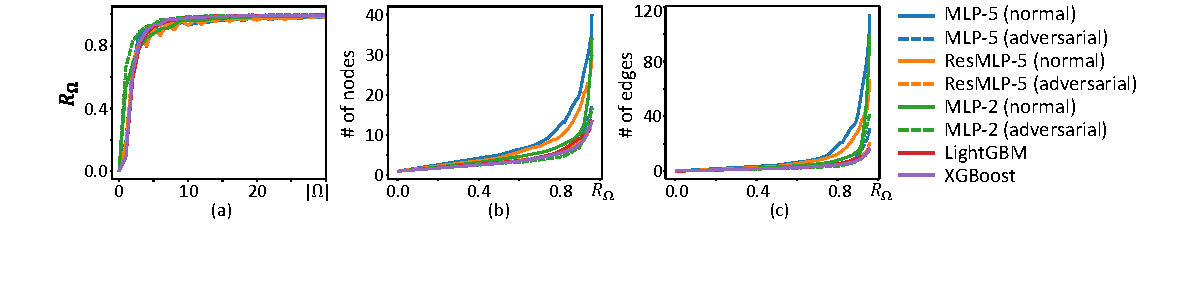
\includegraphics[width=.9\linewidth]{figs/appendix/more-rk-results-census.pdf}
    \caption{(a) The relationship between the number of causal patterns {\small$|\Omega|$} in the AOG and the ratio of the explained causal effects {\small$R_\Omega$}, based on the census dataset. The relationship between {\small$R_\Omega$} and (b) the number of nodes, and (c) the number of edges in the AOG, based on the census dataset.}
    \label{fig:app-rk-census}
\end{figure}
\begin{figure}[t]
    \centering
    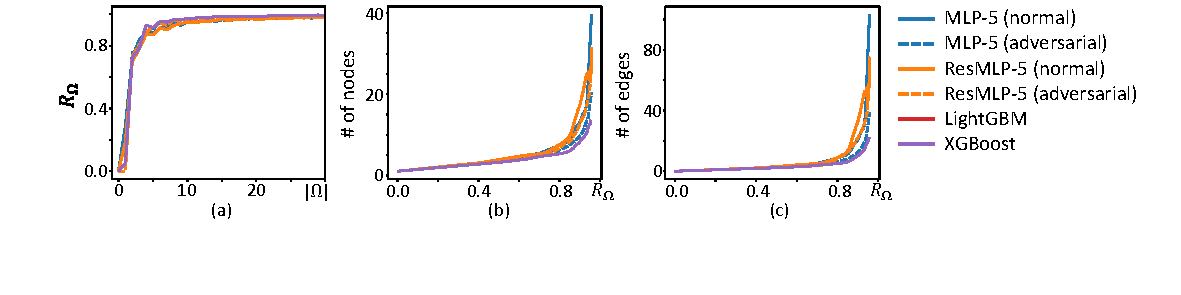
\includegraphics[width=.9\linewidth]{figs/appendix/more-rk-results-bike.pdf}
    \caption{(a) The relationship between the number of causal patterns {\small$|\Omega|$} in the AOG and the ratio of the explained causal effects {\small$R_\Omega$}, based on the bike dataset. The relationship between {\small$R_\Omega$} and (b) the number of nodes, and (c) the number of edges in the AOG, based on the bike dataset.}
    \label{fig:app-rk-bike}
\end{figure}

\subsection{More experimental results on the ratio of the explained causal effects {\small$R_\Omega$}}
\label{sec:app-more-rk}

This section provides more experimental results on the relationship between the ratio of explained causal effects {\small$R_\Omega$} and the AOG explainer.

Similar to the experiment in the Paragraph \textit{Ratio of the explained causal effects}, Section 4.2 of the main paper, we used causal patterns in {\small$\Omega$} to approximate the model output.
Figure \ref{fig:app-rk-census}(a) and Figure \ref{fig:app-rk-bike}(a) show the relationship between {\small$|\Omega|$} and the ratio of explained causal effects {\small$R_\Omega$} in different models, based on the census and bike datasets.
We found that when we used a few causal patterns, we could explain most of the causal effects in the model output.
Figure \ref{fig:app-rk-census}(b,c) and Figure \ref{fig:app-rk-bike}(b,c) show that the node number and edge number increased with the increase in {\small$R_\Omega$}.

Besides, Figure \ref{fig:app-rk-census}(a) and Figure \ref{fig:app-rk-bike} also show that compared with the normally trained model, we could use fewer causal patterns (smaller {\small$|\Omega|$}) to achieve the same ratio of the explained causal effects {\small$R_\Omega$} in the adversarially trained model.
Moreover, Figure \ref{fig:app-rk-census}(b,c) and Figure~\ref{fig:app-rk-bike}(b,c) also show that the AOGs corresponding to adversarially trained models were less complex than the AOGs corresponding to normally trained models.
This indicated that \textit{adversarial training made models encode sparser causal patterns than normal training}.


\subsection{More analysis on the effectiveness of the learned baseline values}
\label{sec:app-effectiveness-baseline-value}

\begin{figure}[t]
    \centering
    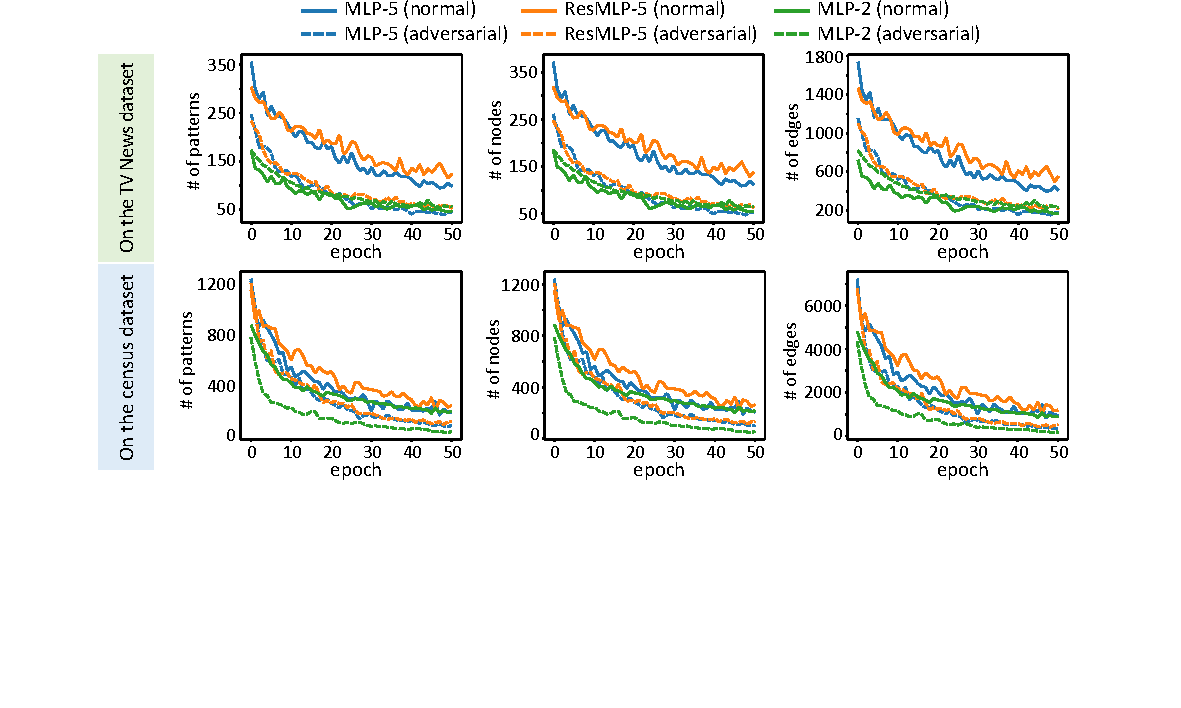
\includegraphics[width=.9\linewidth]{figs/appendix/baseline-value-effect.pdf}
    \caption{The number of patterns (the first column), nodes (the second column), and edges (the third column) in the AOG, based on baseline values of different learning epochs. The learned baseline value significantly enhanced the conciseness of explanations.}
    \label{fig:app-baseline-value-effect}
\end{figure}

This section provides experimental analysis of the effects of baseline values on the conciseness of explanations.
In addition to the experiments in the Paragraph \textit{Effects of baseline values on the conciseness of explanations} in Section~4.2 of the main paper, in this section, we analyze the effectiveness of the learned baseline values in terms of the AOG complexity from different perspectives.
To this end, we first computed causal effects using the baseline values obtained in different epochs during the learning phase.
Then, based on the computed causal effects, we measured the numbers of causal patterns, nodes, and edges in the AOG at each learning epoch.
For a fair comparison, we selected the minimum number {\small$|\Omega|$} of causal patterns such that the ratio of the explained causal effects {\small$Q_\Omega$} exceeded 70\%, to construct the AOG.
Figure \ref{fig:app-baseline-value-effect} shows the change in the AOG complexity during the learning process of baseline values, in terms of the number of causal patterns, nodes, and edges in the AOG.
We found that learning the  baseline values significantly simplified the AOG, thus boosting the conciseness of the explanations.

\subsection{Comparing the complexity of AOGs and the complexity of DNNs}
In this subsection, we compare the complexity of AOGs and the complexity of DNNs.
We trained ResMLP networks with different numbers of layers on the Add-Mul and census datasets, and we explained these DNNs using AOGs. 
Figure~\ref{fig:compare_complexity} shows a comparison of the node number (complexity) of the AOG with the depth and parameter number (complexity) of the DNN. We found that a more complex DNN did not necessarily encode more complex features and thereby did not always obtaining a more complex AOG.

\begin{figure}
    \centering
    \begin{minipage}{0.45\linewidth}
        \centering
        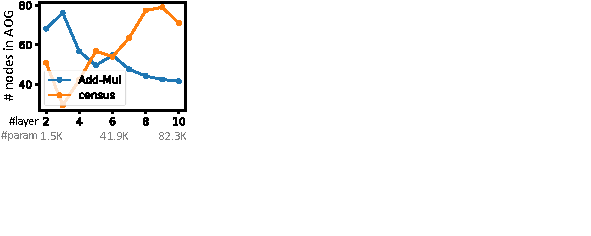
\includegraphics[width=0.5\linewidth]{figs/appendix/rebuttal_DNN_depth_AOG_n_node.pdf}
        \caption{Comparing the complexity (the node number) of the AOG and the complexity (the parameter number) of the DNN.}
        \label{fig:compare_complexity}
    \end{minipage}
\end{figure}


\section{Discussion about the running time of the AOG explainer}

In this section, we conducted an experiment to measure the running time of the methods in Table 2, Section 4.1 of the main paper.
Specifically, we measured the average running time to compute the explanation of a single sample for MLP-5 trained on the census dataset. 
The running time was averaged over 20 different input samples. 
Table~\ref{tab:app-running-time} shows that the proposed AOG explainer was comparable to the existing methods in terms of time complexity.
For the implementation, we implemented the Harsanyi dividend, the Shapley value~\cite{shapley1953value}, the Shapley interaction index~\cite{grabisch1999axiomatic}, and the Shapley Taylor interaction index~\cite{sundararajan2020shapley} by ourselves, and implemented the other three methods (Input{\small$\times$}Gradient~\cite{shrikumar2016not}, LRP~\cite{bach2015pixel}, and Occlusion~\cite{zeiler2014visualizing}) based on the Captum~\cite{kokhlikyan2020captum} package.
All the computation was conducted using an NVIDIA GeForce RTX 2080 Ti GPU. 

\begin{table}[h]
\caption{The average running time to compute the explanation of a single sample, based on different methods.}
\label{tab:app-running-time}
\vspace{-8pt}
\centering
\resizebox{\textwidth}{!}{
\begin{tabular}{c|cccccccc}
\hline
Method & SI & STI ($k=2$) & STI ($k=3$) & Shapley & IxG & LRP & Occ & Ours \\ \hline
Running time (s) & $0.0179{\scriptsize\pm0.0013}$ & $0.0176{\scriptsize\pm1.6 \times10^{-5}}$ & $0.0176{\scriptsize\pm3.9\times10^{-5}}$ & $0.0179{\scriptsize\pm0.0019}$ & $0.0045{\scriptsize\pm0.0014}$ & $0.0170{\scriptsize\pm0.0007}$ & $0.0302{\scriptsize\pm0.0018}$ & $0.0182{\scriptsize\pm0.0010}$ \\ \hline
\end{tabular}
}
\end{table}

For high-dimensional inputs such as images, there are many techniques to solve the dimension problem and reduce the time cost. For example, we can manually segment an input into multiple parts, and use these parts as input variables to construct the AOG. 
In this way, the running time required to compute an AOG on the CelebA dataset was reduced to 4.03 s.
Besides, we can also ignore casual patterns between distant parts to accelerate the computation.



\section{Discussion about the difference between the AOG explainer and the BoW model}

\textbf{Do we explain a DNN as a linear model, such as a bag-of-words (BoW) model~\cite{sivic2003video,csurka2004visual}?}
First, although the AOG explainer appears to be a linear additive model, the AOG explainer does NOT simplify the non-linear deep model as a linear model.
Instead, as mentioned in Section~3.1 of the main paper, the AOG explainer extracts different causal patterns from different input samples, instead of using the same set of causal patterns to explain different samples.
It is because the deep model is non-linear and triggers different causal patterns to handle different samples.
Therefore, unlike the BoW model, which extracts the same set of features for each sample, the AOG explainer quantifies the manner in which the deep model triggers different causal patterns to handle different samples, thereby remaining non-linear for different inputs.
Second, the BoW model considers only the presence or absence of input variables, whereas the AOG explainer is sensitive to the spatial relationships of input variables.
For example, Table \ref{tab:aog-bow-1} shows the causal effects {\small$w_{\mathcal{S}}$} of the same sets of words {\small$\mathcal{S}$} encoded by the deep model\footnote{In this example, we explained the causal effects encoded by a two-layer LSTM model trained on the SST-2 dataset for sentiment classification. We set {\small$v(\boldsymbol{x}_{\mathcal{S}}) =p(y=\text{positive sentiment}|\boldsymbol{x}_{\mathcal{S}})$}.}, given two sentences with the same words but different word positions.
We found that the deep model encoded significantly different causal effects between the same sets of words, demonstrating that the AOG explainer differs from the BoW model.




\begin{table}[htbp]
\centering
\caption{Given two sentences with the same words but different word positions, the causal effects of the same sets of words {\small$\mathcal{S}$} encoded by the deep model were different. 
This demonstrated that the AOG explainer was sensitive to the spatial relationship of input variables, indicating a difference with the BoW model.}
\label{tab:aog-bow-1}
\resizebox{.65\textwidth}{!}{
\begin{tabular}{cccc}
\hline
\multicolumn{2}{c}{Sentence 1: it's just not very smart.} & \multicolumn{2}{c}{Sentence 2: it's not just very smart.} \\
sets of words {\small$\mathcal{S}$} & causal effects {\small$w_{\mathcal{S}}$} & sets of words {\small$\mathcal{S}$} & causal effects {\small$w_{\mathcal{S}}$} \\ \hline
{\small$\{\textit{just, not, smart, .}\}$} & -1.616 & {\small$\{\textit{not, just, smart, .}\}$} & 1.139 \\ \hline
{\small$\{\textit{it, just, not, very}\}$} & -1.510 & {\small$\{\textit{it, not, just, very}\}$} & 5.908 \\ \hline
{\small$\{\textit{'s, just, not, very, smart}\}$} & -1.172 & {\small$\{\textit{'s, not, just, very, smart}\}$} & 0.890 \\ \hline
{\small$\{\textit{just, not, very, smart}\}$} & -0.715 & {\small$\{\textit{not, just, very, smart}\}$} & 3.563 \\ \hline
\end{tabular}
}
\end{table}


Nevertheless, common and salient causal patterns shared by different input samples can also be considered the basic elementary concepts encoded by the deep model.
For example, if two sentences contain the same set of words {\small$\mathcal{S}$} in the same position, then the deep model encodes the same causal effects {\small$ w_{\mathcal{S}'} ,\forall \mathcal{S}'\subseteq \mathcal{S}$}.
Table \ref{tab:aog-bow-2} shows that the deep model encoded the same causal effects within {\small$\mathcal{S}=\{\textit{not, very, smart}\}$} for two different sentences.
From this perspective, such common causal patterns can be roughly  considered as typical ``words'' in a BoW model.


\begin{table}[htbp]
\centering
\caption{Given two sentences containing the same set of words {\small$\mathcal{S}=\{\textit{not, very, smart}\}$}, the causal effects within the subset of words {\small$\mathcal{S}$} encoded by the deep model were the same. The deep model encoded the same causal effects {\small$w_{\mathcal{S}'} ,\forall \mathcal{S}'\subseteq \mathcal{S}$}.}
\label{tab:aog-bow-2}
\resizebox{.6\textwidth}{!}{
\begin{tabular}{cccc}
\hline
\multicolumn{2}{c}{Sentence 1: it's just not very smart.} & \multicolumn{2}{c}{Sentence 3: he is just not very smart.} \\
sets of words {\small$\mathcal{S}'\subseteq \mathcal{S}$} & causal effect {\small$w_{\mathcal{S}'}$} & sets of words {\small$\mathcal{S}'\subseteq \mathcal{S}$} & causal effect {\small$w_{\mathcal{S}'}$} \\ \hline
{\small$\{\textit{not, smart}\}$} & -13.481 & {\small$\{\textit{not, smart}\}$} & -13.481 \\ \hline
{\small$\{\textit{not, very}\}$} & -12.826 & {\small$\{\textit{not, very}\}$} & -12.826 \\ \hline
{\small$\{\textit{smart}\}$} & 6.568 & {\small$\{\textit{smart}\}$} & 6.568 \\ \hline
{\small$\{\textit{very, smart}\}$} & 3.720 & {\small$\{\textit{very, smart}\}$} & 3.720 \\ \hline
{\small$\{\textit{not}\}$} & 0.939 & {\small$\{\textit{not}\}$} & 0.939 \\ \hline
{\small$\{\textit{not, very, smart}\}$} & 0.837 & {\small$\{\textit{not, very, smart}\}$} & 0.837 \\ \hline
{\small$\{\textit{very}\}$} & -0.197 & {\small$\{\textit{very}\}$} & -0.197 \\ \hline
\end{tabular}
}
\end{table}


\newpage

\begin{figure}[p]
    \centering
    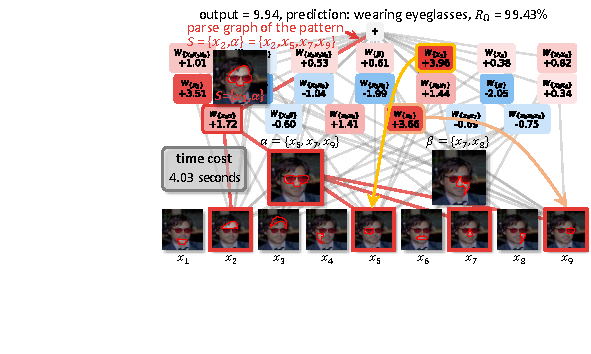
\includegraphics[width=0.6\linewidth]{figs/appendix/rebuttal_CelebA_AOG.pdf}
    \caption{An examples of AOGs extracted from the ResNet-18 network, trained on the CelebA dataset.}
    \label{fig:aog-celeba-resnet18}
\end{figure}

\begin{figure}[p]
    \centering
    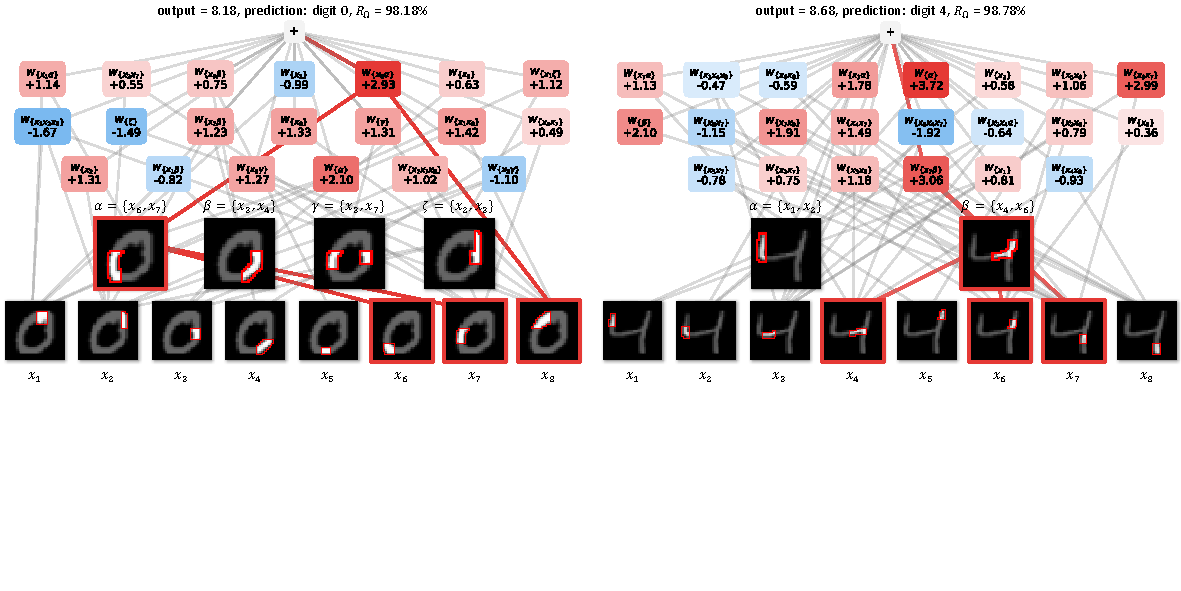
\includegraphics[width=\linewidth]{figs/appendix/aog-resnet32-mnist.pdf}
    \caption{Examples of AOGs extracted from the ResNet-32 network, trained on the MNIST dataset.}
    \label{fig:aog-mnist-resnet32}
\end{figure}

\begin{figure}[p]
    \centering
    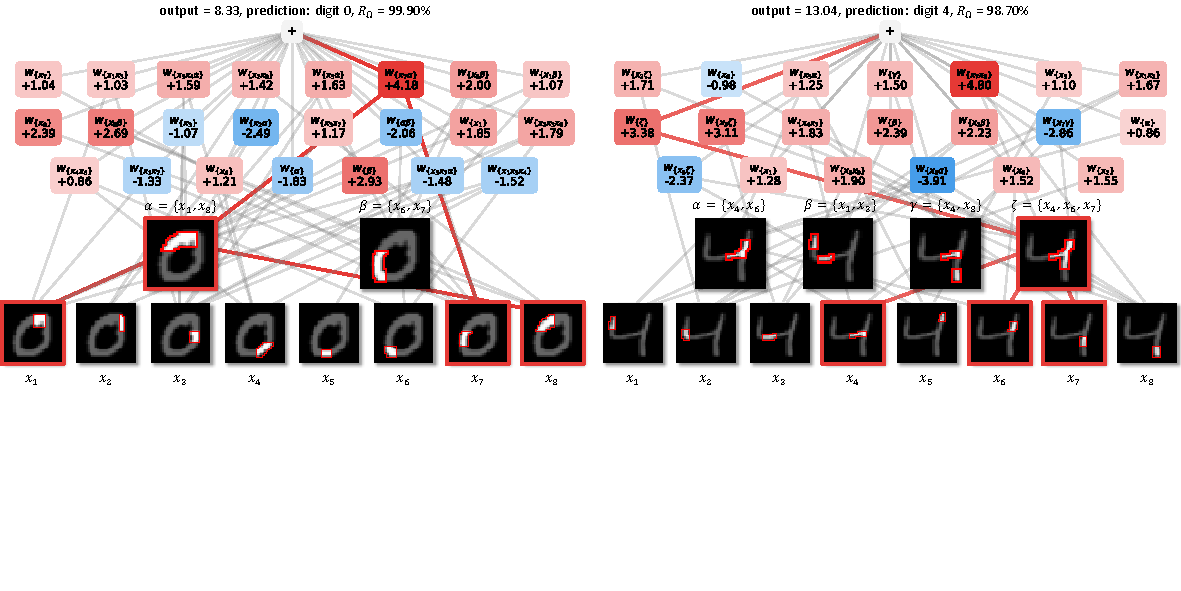
\includegraphics[width=\linewidth]{figs/appendix/aog-resnet44-mnist.pdf}
    \caption{Examples of AOGs extracted from the ResNet-44 network, trained on the MNIST dataset.}
    \label{fig:aog-mnist-resnet44}
\end{figure}

\begin{figure}[p]
    \centering
    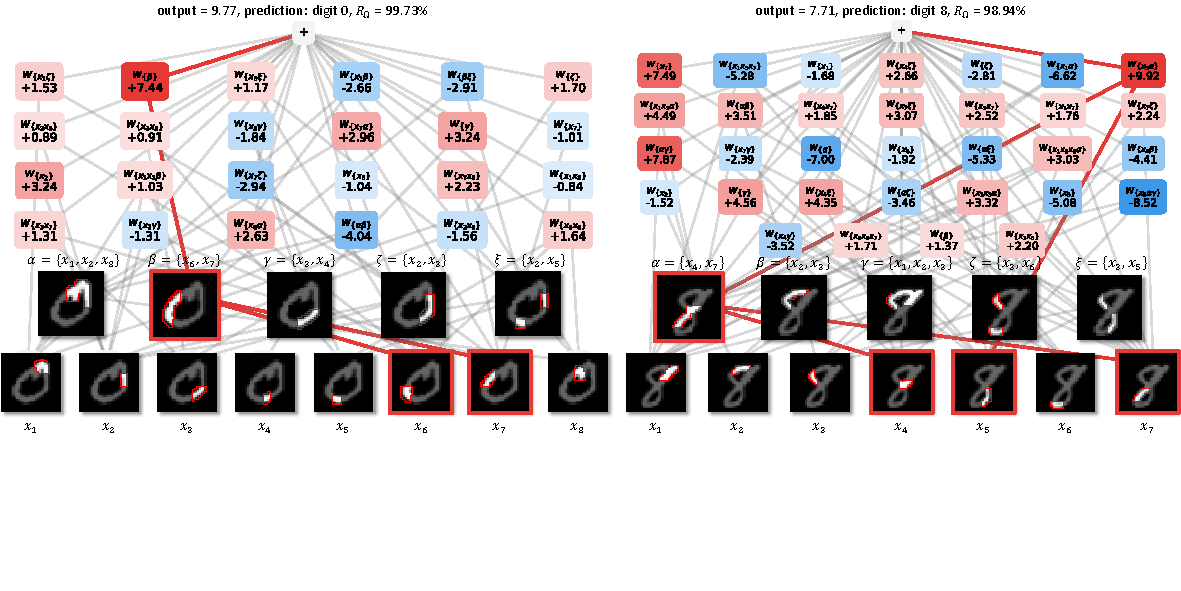
\includegraphics[width=\linewidth]{figs/appendix/aog-vgg16-mnist.pdf}
    \caption{Examples of AOGs extracted from the VGG-16 network, trained on the MNIST dataset.}
    \label{fig:aog-mnist-vgg16}
\end{figure}

\begin{figure}[p]
    \centering
    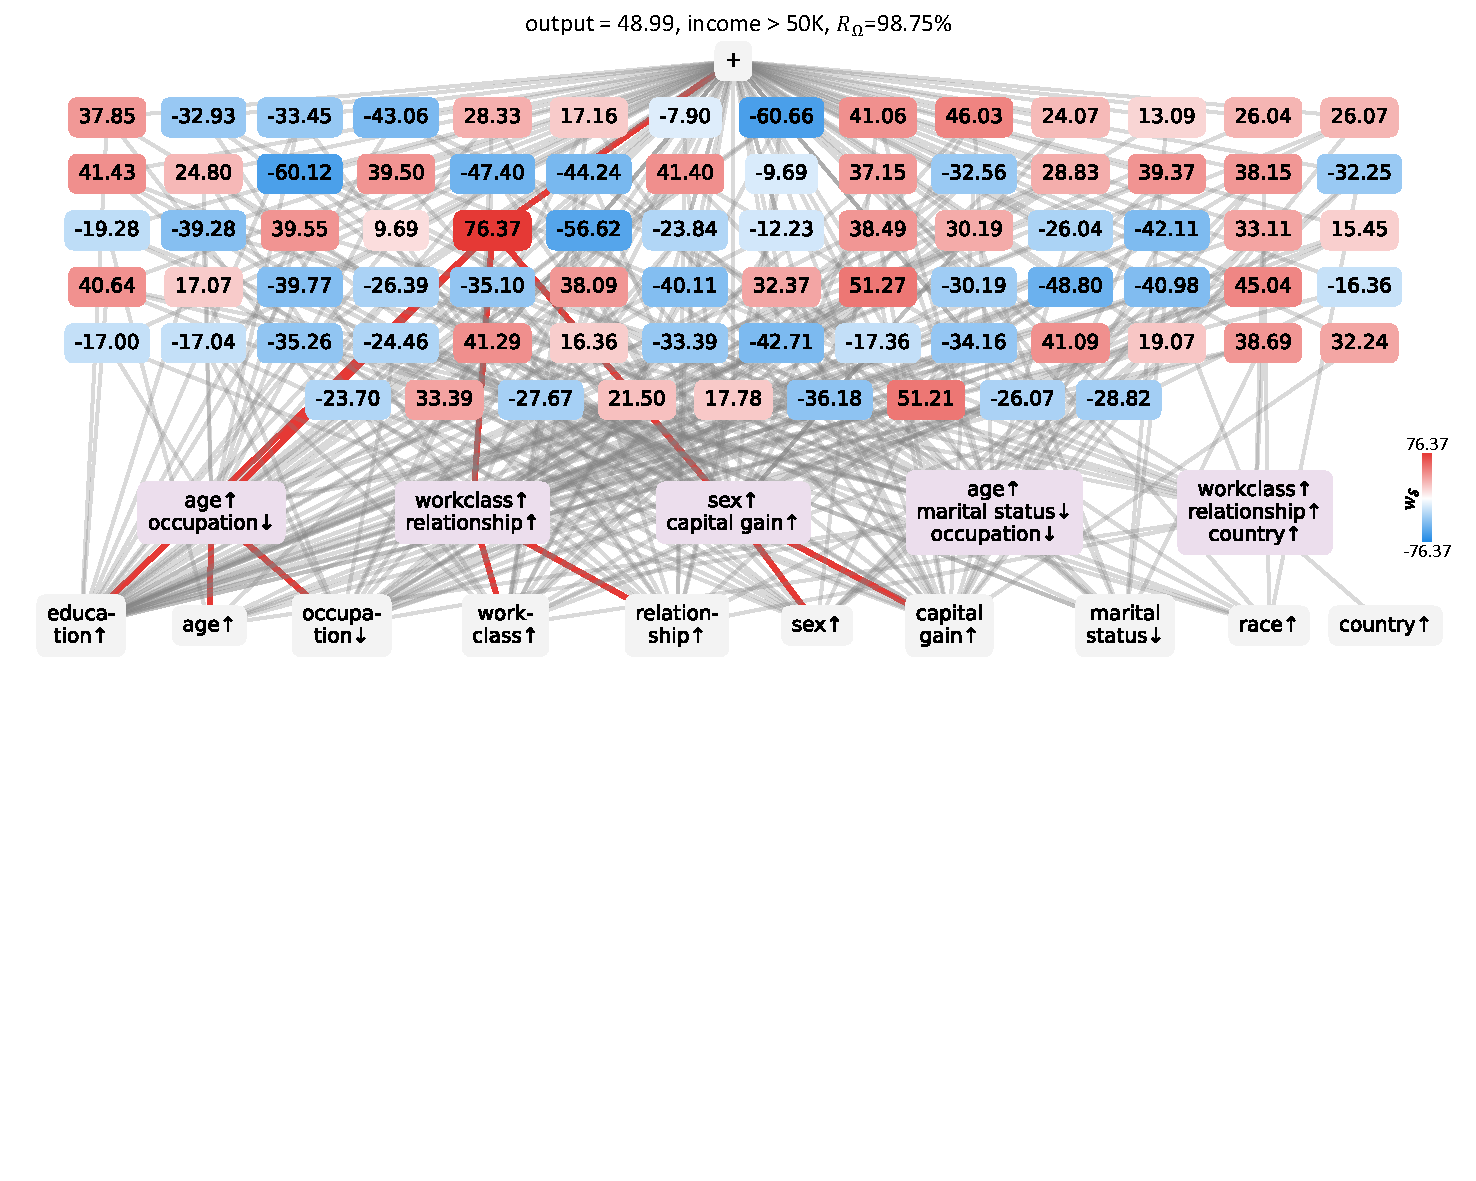
\includegraphics[width=\linewidth]{figs/appendix/aog-census-mlp5-big.pdf}
    \caption{An example of the AOG extracted from the MLP-5 network, trained on the census dataset. Red edges indicate the parse graph of the most salient causal pattern.}
    \label{fig:aog-census-mlp5-normal}
\end{figure}

\begin{figure}[p]
    \centering
    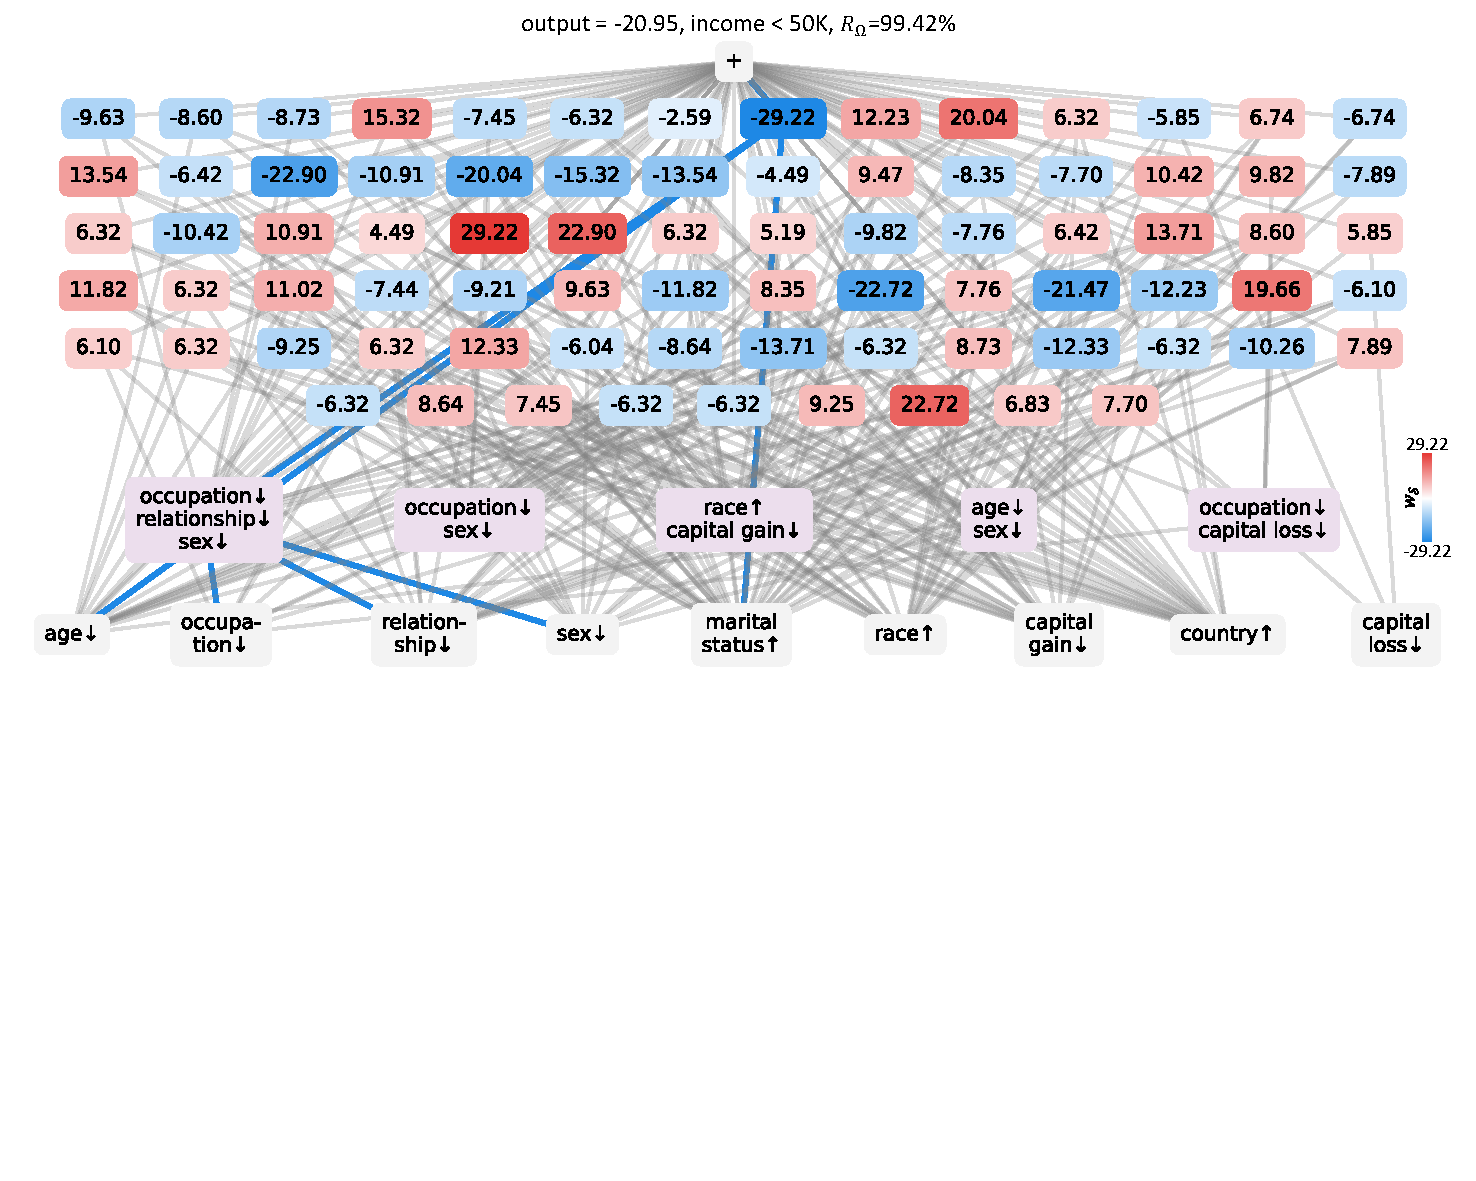
\includegraphics[width=\linewidth]{figs/appendix/aog-census-resmlp5-big.pdf}
    \caption{An example of the AOG extracted from the ResMLP-5 network, trained on the census dataset. Red edges indicate the parse graph of the most salient causal pattern.}
    \label{fig:aog-census-resmlp5-normal}
\end{figure}

\begin{figure}[h]
    \centering
    \begin{subfigure}{\linewidth}
        \centering
        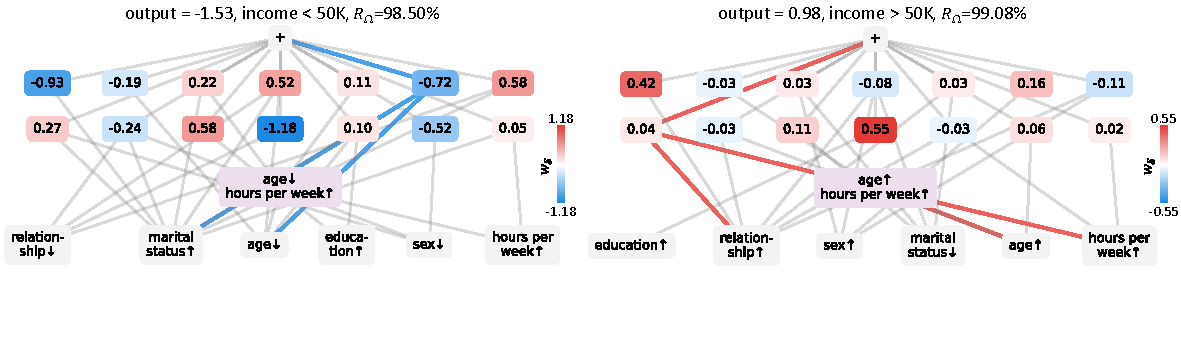
\includegraphics[width=.95\linewidth]{figs/appendix/aog-census-mlp2-adv.pdf}
        \caption{Examples of AOGs extracted from the MLP-2 network, adversarially trained on the census dataset.}
        \vspace{10pt}
    \end{subfigure}
    \begin{subfigure}{\linewidth}
        \centering
        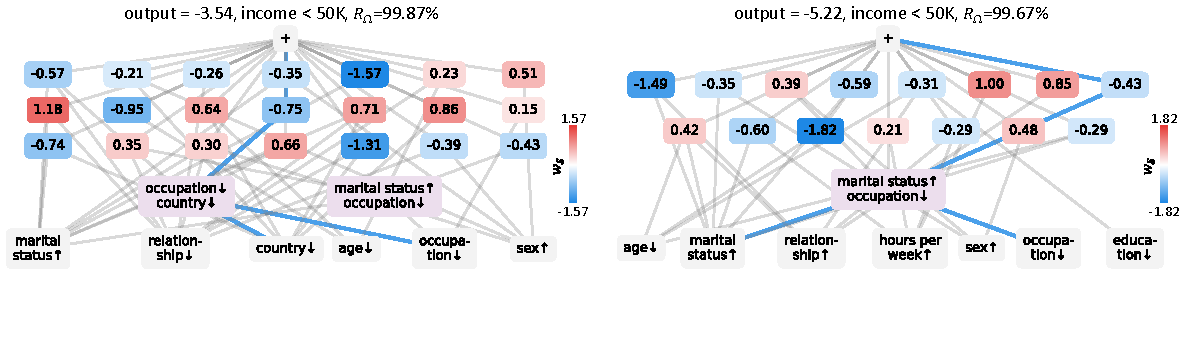
\includegraphics[width=.95\linewidth]{figs/appendix/aog-census-mlp5-adv.pdf}
        \caption{Examples of AOGs extracted from the MLP-5 network, adversarially trained on the census dataset.}
        \vspace{10pt}
    \end{subfigure}
    \begin{subfigure}{\linewidth}
        \centering
        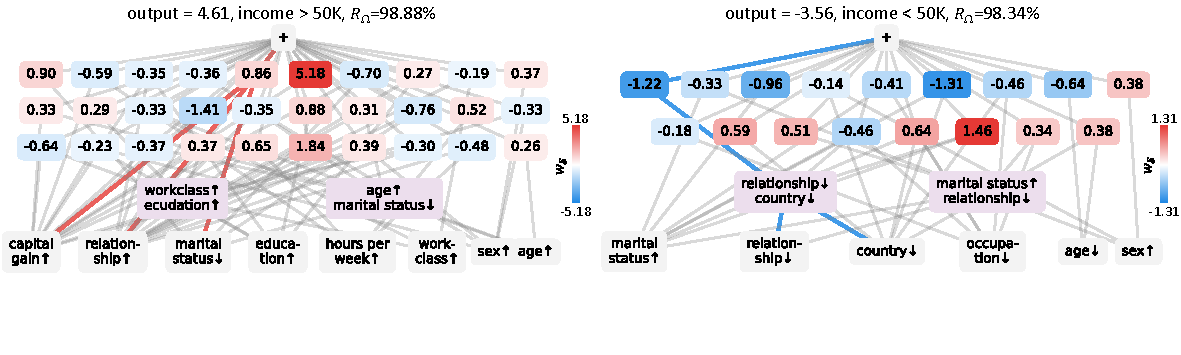
\includegraphics[width=.95\linewidth]{figs/appendix/aog-census-resmlp5-adv.pdf}
        \caption{Examples of AOGs extracted from the ResMLP-5 network, adversarially trained on the census dataset.}
    \end{subfigure}
    \caption{Examples of AOGs extracted from models trained on the census dataset. Red edges indicate the parse graph of a specific causal pattern.}
    \label{fig:aog-census}
\end{figure}

\begin{figure}[h]
    \centering
    \begin{subfigure}{\linewidth}
        \centering
        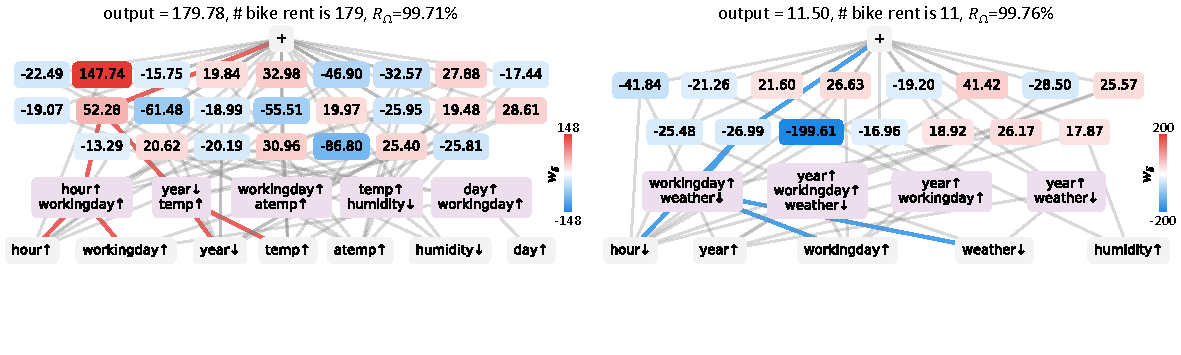
\includegraphics[width=.95\linewidth]{figs/appendix/aog-bike-mlp5-adv.pdf}
        \caption{Examples of AOGs extracted from the MLP-5 network, adversarially trained on the bike dataset.}
    \end{subfigure}
\end{figure}

\begin{figure}[h]\ContinuedFloat
    \begin{subfigure}{\linewidth}
        \centering
        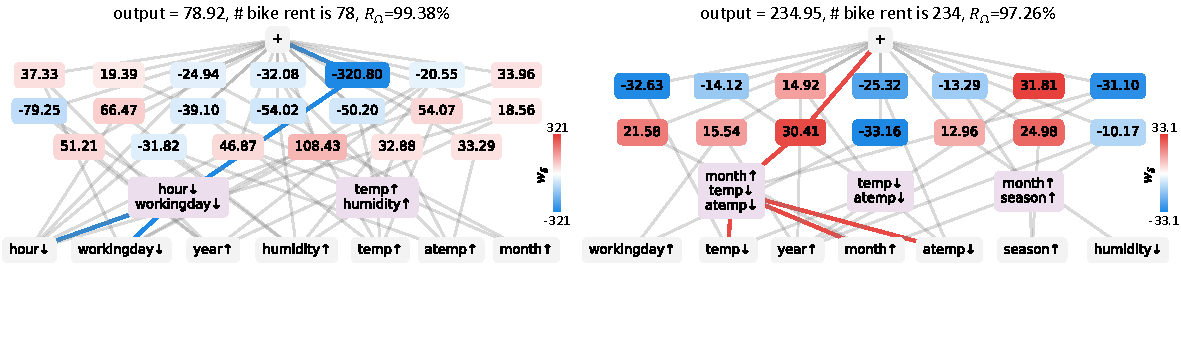
\includegraphics[width=.95\linewidth]{figs/appendix/aog-bike-resmlp5-adv.pdf}
        \caption{Examples of AOGs extracted from the ResMLP-5 network, adversarially trained on the bike dataset.}
    \end{subfigure}
    \caption{Examples of AOGs extracted from models trained on the bike dataset. Red edges indicate the parse graph of a specific causal pattern.}
    \label{fig:aog-bike}
\end{figure}


\begin{figure}[h]
    \centering
    \begin{subfigure}{\linewidth}
        \centering
        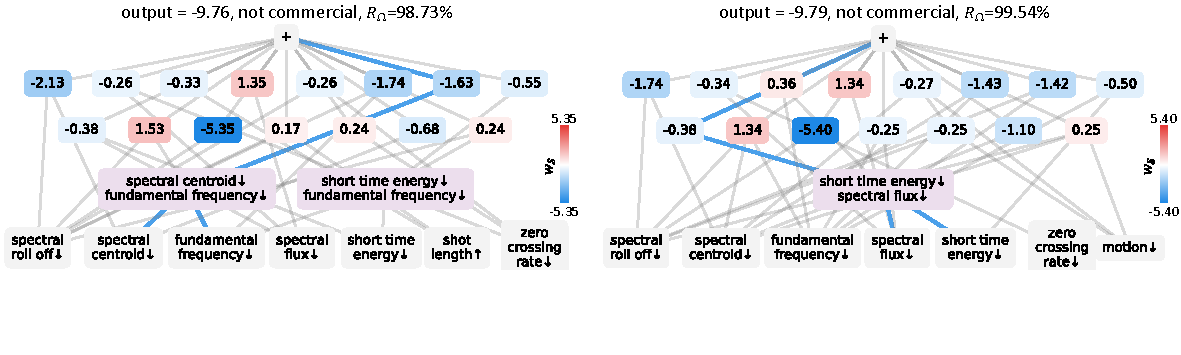
\includegraphics[width=.95\linewidth]{figs/appendix/aog-commercial-mlp2-adv.pdf}
        \caption{Examples of AOGs extracted from the MLP-2 network, adversarially trained on the TV news dataset.}
    \end{subfigure}
    \begin{subfigure}{\linewidth}
        \centering
        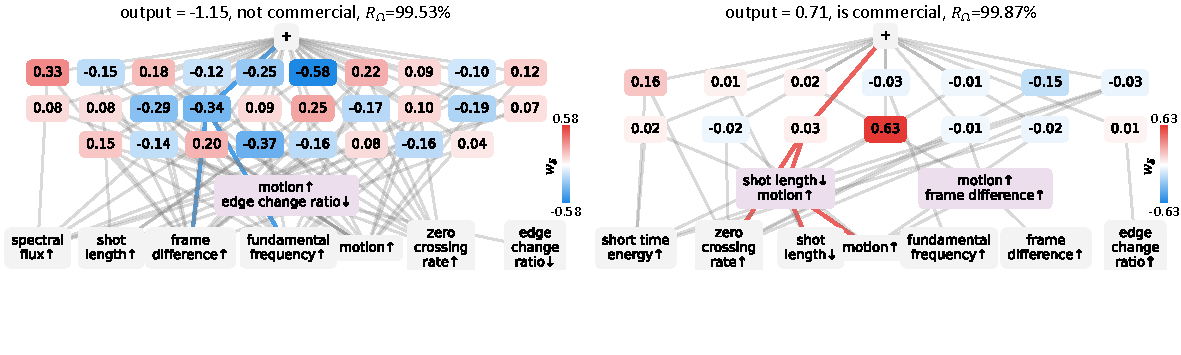
\includegraphics[width=.95\linewidth]{figs/appendix/aog-commercial-mlp5-adv.pdf}
        \caption{Examples of AOGs extracted from the MLP-5 network, adversarially trained on the TV news dataset.}
    \end{subfigure}
    \begin{subfigure}{\linewidth}
        \centering
        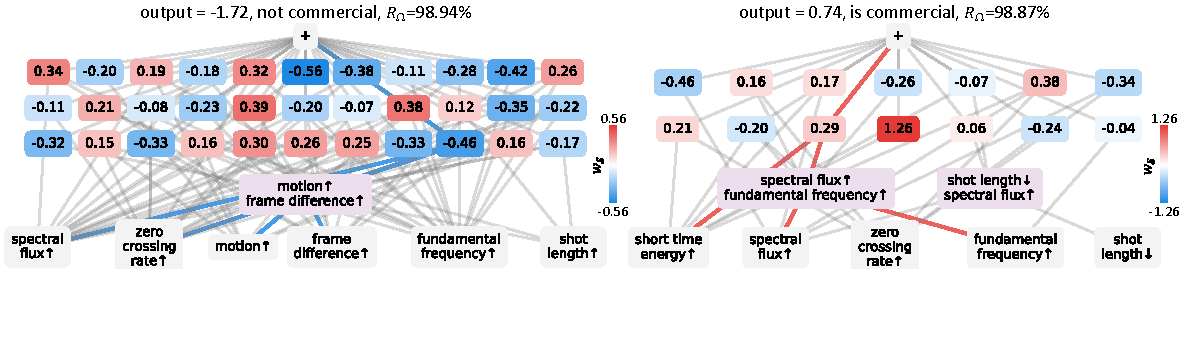
\includegraphics[width=.95\linewidth]{figs/appendix/aog-commercial-resmlp5-adv.pdf}
        \caption{Examples of AOGs extracted from the ResMLP-5 network, adversarially trained on the TV news dataset.}
    \end{subfigure}
    \caption{Examples of AOGs extracted from models trained on the TV news dataset. Red edges indicate the parse graph of a specific causal pattern.}
    \label{fig:aog-commercial}
\end{figure}


\begin{figure}[h]
    \centering
    \begin{subfigure}{\linewidth}
        \centering
        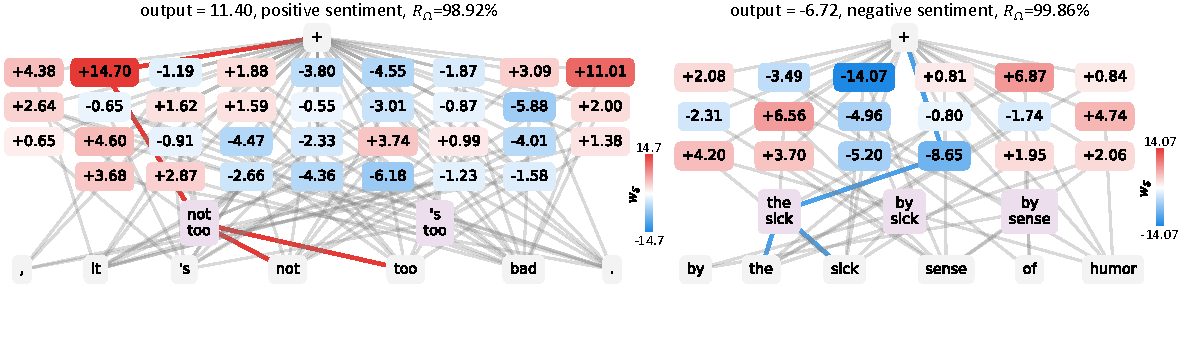
\includegraphics[width=.95\linewidth]{figs/appendix/aog-sst2-cnn.pdf}
        \caption{Examples of AOGs extracted from the CNN network, trained on the SST-2 dataset.}
    \end{subfigure}
    \begin{subfigure}{\linewidth}
        \centering
        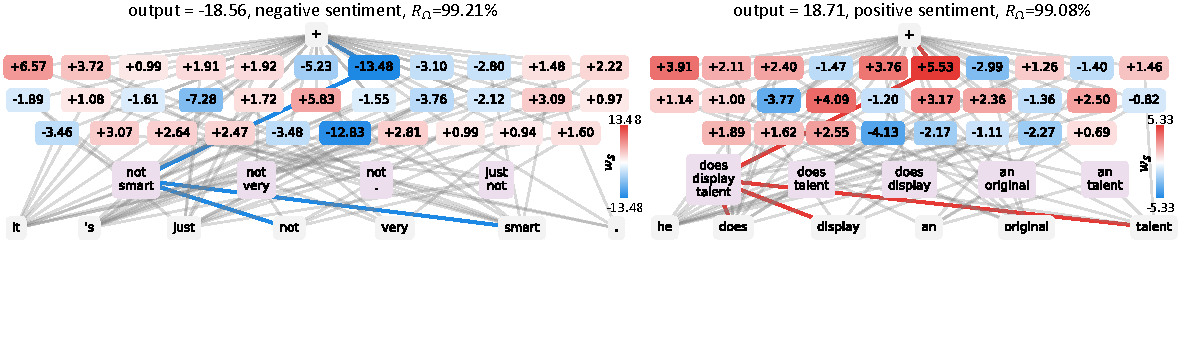
\includegraphics[width=.95\linewidth]{figs/appendix/aog-sst2-lstm.pdf}
        \caption{Examples of AOGs extracted from the LSTM network, trained on the SST-2 dataset.}
    \end{subfigure}
    \caption{Examples of AOGs extracted from models trained on the SST-2 dataset. Red edges indicate the parse graph of the most salient causal pattern.}
    \label{fig:aog-sst2}
\end{figure}

\begin{figure}[h]
    \centering
    \begin{subfigure}{\linewidth}
        \centering
        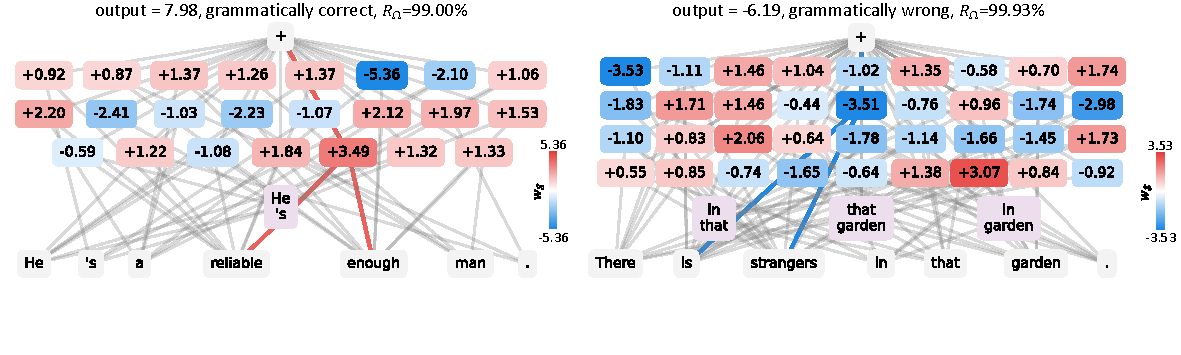
\includegraphics[width=.95\linewidth]{figs/appendix/aog-cola-cnn.pdf}
        \caption{Examples of AOGs extracted from the CNN network, trained on the CoLA dataset.}
    \end{subfigure}
    \begin{subfigure}{\linewidth}
        \centering
        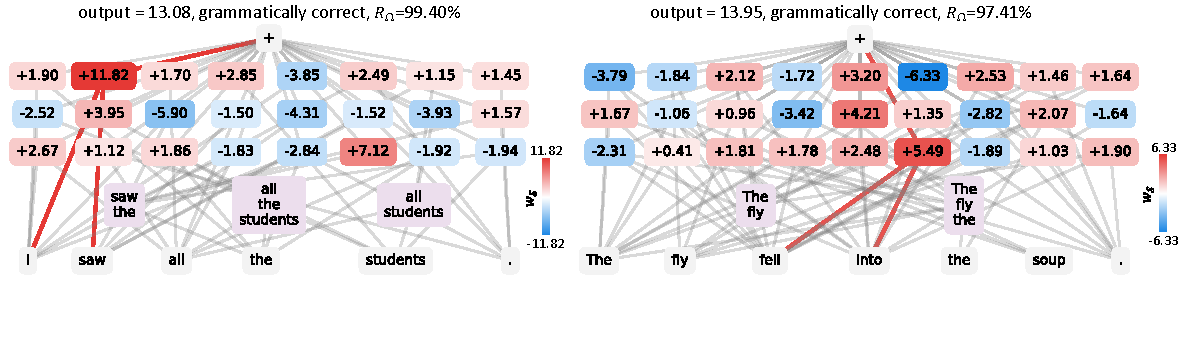
\includegraphics[width=.95\linewidth]{figs/appendix/aog-cola-lstm.pdf}
        \caption{Examples of AOGs extracted from the LSTM network, trained on the CoLA dataset.}
    \end{subfigure}
    \caption{Examples of AOGs extracted from models trained on the CoLA dataset. Red edges indicate the parse graph of the most salient causal pattern.}
    \label{fig:aog-cola}
\end{figure}

\begin{figure}[h]
    \centering
    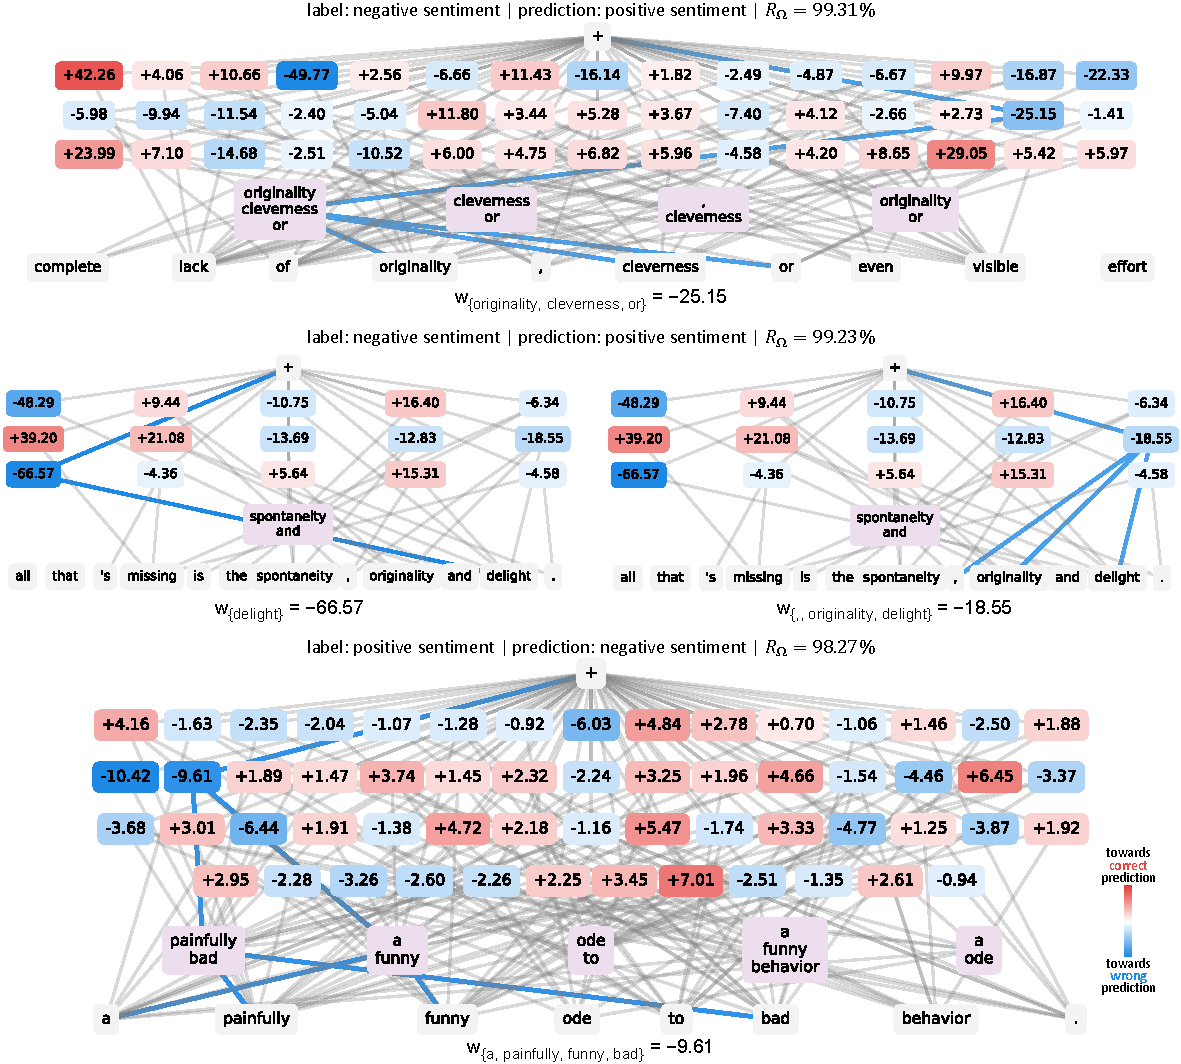
\includegraphics[width=\linewidth]{figs/appendix/misclassified-more.pdf}
    \caption{AOGs that explained incorrect predictions of the network model trained on the SST-2 dataset. Red edges indicated the parse graphs of causal patterns towards correct predictions, while blue edges indicated parse graphs of causal patterns towards wrong predictions.}
    \label{fig:misclassified-more}
\end{figure}

